% Options for packages loaded elsewhere
\PassOptionsToPackage{unicode}{hyperref}
\PassOptionsToPackage{hyphens}{url}
\documentclass[
]{book}
\usepackage{xcolor}
\usepackage{amsmath,amssymb}
\setcounter{secnumdepth}{-\maxdimen} % remove section numbering
\usepackage{iftex}
\ifPDFTeX
  \usepackage[T1]{fontenc}
  \usepackage[utf8]{inputenc}
  \usepackage{textcomp} % provide euro and other symbols
\else % if luatex or xetex
  \usepackage{unicode-math} % this also loads fontspec
  \defaultfontfeatures{Scale=MatchLowercase}
  \defaultfontfeatures[\rmfamily]{Ligatures=TeX,Scale=1}
\fi
\usepackage{lmodern}
\ifPDFTeX\else
  % xetex/luatex font selection
\fi
% Use upquote if available, for straight quotes in verbatim environments
\IfFileExists{upquote.sty}{\usepackage{upquote}}{}
\IfFileExists{microtype.sty}{% use microtype if available
  \usepackage[]{microtype}
  \UseMicrotypeSet[protrusion]{basicmath} % disable protrusion for tt fonts
}{}
\makeatletter
\@ifundefined{KOMAClassName}{% if non-KOMA class
  \IfFileExists{parskip.sty}{%
    \usepackage{parskip}
  }{% else
    \setlength{\parindent}{0pt}
    \setlength{\parskip}{6pt plus 2pt minus 1pt}}
}{% if KOMA class
  \KOMAoptions{parskip=half}}
\makeatother
\usepackage{graphicx}
\makeatletter
\newsavebox\pandoc@box
\newcommand*\pandocbounded[1]{% scales image to fit in text height/width
  \sbox\pandoc@box{#1}%
  \Gscale@div\@tempa{\textheight}{\dimexpr\ht\pandoc@box+\dp\pandoc@box\relax}%
  \Gscale@div\@tempb{\linewidth}{\wd\pandoc@box}%
  \ifdim\@tempb\p@<\@tempa\p@\let\@tempa\@tempb\fi% select the smaller of both
  \ifdim\@tempa\p@<\p@\scalebox{\@tempa}{\usebox\pandoc@box}%
  \else\usebox{\pandoc@box}%
  \fi%
}
% Set default figure placement to htbp
\def\fps@figure{htbp}
\makeatother
\setlength{\emergencystretch}{3em} % prevent overfull lines
\providecommand{\tightlist}{%
  \setlength{\itemsep}{0pt}\setlength{\parskip}{0pt}}
\usepackage{bookmark}
\IfFileExists{xurl.sty}{\usepackage{xurl}}{} % add URL line breaks if available
\urlstyle{same}
\hypersetup{
  hidelinks,
  pdfcreator={LaTeX via pandoc}}

\author{}
\date{}

\begin{document}
\frontmatter

\mainmatter
\chapter{Menggambar Grafik 2D dengan EMT}\label{menggambar-grafik-2d-dengan-emt}

Notebook ini menjelaskan tentang cara menggambar berbagai kurva dan grafik 2D dengan software EMT. EMT menyediakan fungsi plot2d() untuk menggambar berbagai kurva dan grafik dua dimensi (2D).

\section{Plot Dasar}\label{plot-dasar}

Ada fungsi plot yang sangat mendasar. Terdapat koordinat layar yang selalu berkisar antara 0 hingga 1024 di setiap sumbu, tidak peduli apakah layarnya berbentuk persegi atau tidak. Dan terdapat koordinat plot yang dapat diatur dengan setplot(). Pemetaan antar koordinat bergantung pada jendela plot saat ini. Misalnya, bawaan shrinkwindow() menyisakan ruang untuk label sumbu dan judul plot.

Dalam contoh ini, kita hanya menggambar beberapa garis acak dengan berbagai warna. Untuk rincian tentang fungsi-fungsi ini, pelajari fungsi inti EMT.

\textgreater clg; // untuk membersihkan layar

\textgreater window(0,0,1024,1024); // menggunakan seluruh jendela

\textgreater setplot(0,1,0,1); // mengatur koordinat plot

\textgreater hold on;

hold on digunakan untuk memulai mode overwrite atau menimpa sehingga grafik yang baru akan ditambahkan ke grafik yang sudah ada

\textgreater n=100; X=random(n,2); Y=random(n,2); // mendapatkan titik random

\textgreater colors=rgb(random(n),random(n),random(n)); // mendapatkan warna random

\textgreater loop 1 to n; color(colors{[}\#{]}); plot(X{[}\#{]},Y{[}\#{]}); end; // plot

\textgreater hold off; // mengakhiri mode overwrite

\textgreater insimg; // memasukkan ke notebook

\begin{figure}
\centering
\pandocbounded{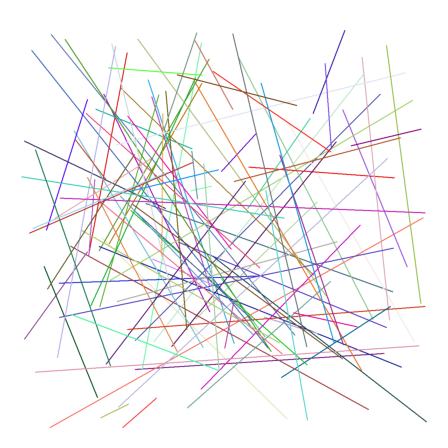
\includegraphics[keepaspectratio]{images/EMT4Plot2D - Naila Khalidatus Salwa-001.png}}
\caption{images/EMT4Plot2D\%20-\%20Naila\%20Khalidatus\%20Salwa-001.png}
\end{figure}

\textgreater reset; //menghapus semua grafik sehingga siap membuat grafik baru

Grafik perlu ditahan, karena perintah plot() akan menghapus jendela plot.

Untuk menghapus semua yang kita lakukan, gunakan reset().

Untuk menampilkan gambar hasil plot di layar notebook, perintah plot2d() dapat diakhiri dengan titik dua (:). Cara lain adalah perintah plot2d() diakhiri dengan titik koma (;), kemudian menggunakan perintah insimg() untuk menampilkan gambar hasil plot.

Contoh lain, kita menggambar plot sebagai sisipan di plot lain. Hal ini dilakukan dengan mendefinisikan jendela plot yang lebih kecil. Perhatikan bahwa jendela ini tidak memberikan ruang untuk label sumbu di luar jendela plot. Kita harus menambahkan beberapa margin untuk ini sesuai kebutuhan. Perhatikan bahwa kita menyimpan dan memulihkan jendela penuh, dan menahan plot saat ini sementara kita memplot inset.

\textgreater plot2d(``x\^{}3-x'');

\textgreater xw=200; yw=100; ww=300; hw=300; //baris ini mengatur koordinat dan ukuran jendela plot

\textgreater ow=window();

ow=

variabel yang akan menimpa plot

\textgreater window(xw,yw,xw+ww,yw+hw);

mengatur jendela dengan posisi dan ukuran yang sudah ditentukan sebelumnya

\textgreater hold on;

\textgreater barclear(xw-50,yw-10,ww+60,ww+60);

fungsi yang mungkin untuk membersihkan di sekitar jendela bersih sebelum menan{]}mbah grafik baru

\textgreater plot2d(``x\^{}4-x'',grid=6):

\begin{figure}
\centering
\pandocbounded{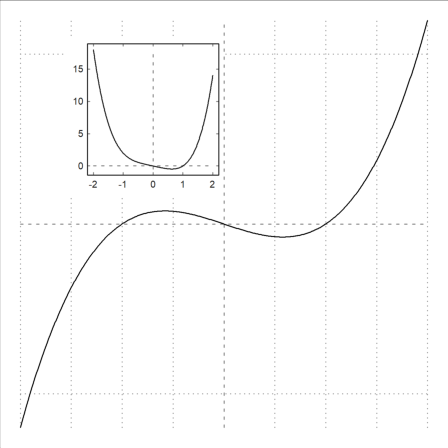
\includegraphics[keepaspectratio]{images/EMT4Plot2D - Naila Khalidatus Salwa-002.png}}
\caption{images/EMT4Plot2D\%20-\%20Naila\%20Khalidatus\%20Salwa-002.png}
\end{figure}

\textgreater hold off;

\textgreater window(ow);//mengembalikan jendela ke keadaan sebelumnya

Plot dengan banyak gambar dicapai dengan cara yang sama. Ada fungsi utilitas figure() untuk ini.

\section{Plot Aspek}\label{plot-aspek}

Plot bawaan menggunakan jendela plot persegi. Anda dapat mengubahnya dengan fungsi aspect(). Jangan lupa untuk mengatur ulang aspeknya nanti. Anda juga dapat mengubah default ini di menu dengan ``Set Aspect'' ke rasio aspek tertentu atau ke ukuran jendela grafik saat ini.

Tapi Anda juga bisa mengubahnya untuk satu plot. Untuk ini, ukuran area plot saat ini diubah, dan jendela diatur sehingga label memiliki cukup ruang.

\textgreater aspect(2); // rasio panjang dan lebar 2:1

\textgreater plot2d({[}``sin(x)'',``cos(x)''{]},0,2pi):

\begin{figure}
\centering
\pandocbounded{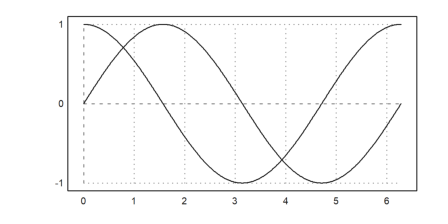
\includegraphics[keepaspectratio]{images/EMT4Plot2D - Naila Khalidatus Salwa-003.png}}
\caption{images/EMT4Plot2D\%20-\%20Naila\%20Khalidatus\%20Salwa-003.png}
\end{figure}

\textgreater aspect();

\textgreater reset;

Fungsi reset() mengembalikan default plot termasuk rasio aspek.

\chapter{Plot 2D di Euler}\label{plot-2d-di-euler}

EMT Math Toolbox memiliki plot dalam 2D, baik untuk data maupun fungsi. EMT menggunakan fungsi plot2d. Fungsi ini dapat memplot fungsi dan data.

Dimungkinkan untuk membuat plot di Maxima menggunakan Gnuplot atau dengan Python menggunakan Math Plot Lib.

Euler dapat membuat plot 2D

\begin{itemize}
\item
  ekspresi
\item
  functions, variables, or parameterized curves,
\item
  vectors of x-y-values,
\item
  clouds of points in the plane,
\item
  implicit curves with levels or level regions.
\item
  Complex function
\end{itemize}

Gaya plot mencakup berbagai gaya untuk garis dan titik, plot batang, dan plot berbayang.

\chapter{Plot Ekspresi atau Variabel}\label{plot-ekspresi-atau-variabel}

Ekspresi tunggal dalam ``x'' (misalnya ``4*x\^{}2'') atau nama suatu fungsi (misalnya ``f'') menghasilkan grafik fungsi tersebut.

Berikut adalah contoh paling dasar, yang menggunakan rentang default dan menetapkan rentang y yang tepat agar sesuai dengan plot fungsinya.

Catatan: Jika Anda mengakhiri baris perintah dengan titik dua ``:'', plot akan dimasukkan ke dalam jendela teks. Jika tidak, tekan TAB untuk melihat plot jika jendela plot tertutup.

\textgreater plot2d(``x\^{}2''):

\begin{figure}
\centering
\pandocbounded{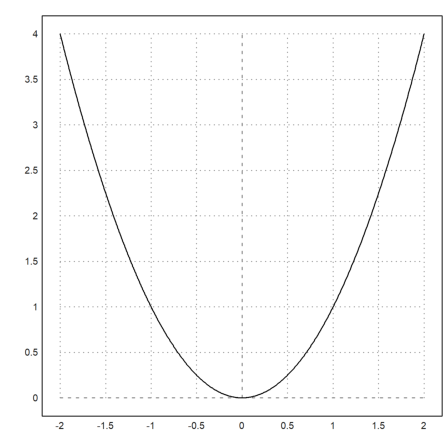
\includegraphics[keepaspectratio]{images/EMT4Plot2D - Naila Khalidatus Salwa-004.png}}
\caption{images/EMT4Plot2D\%20-\%20Naila\%20Khalidatus\%20Salwa-004.png}
\end{figure}

\textgreater aspect(1.5); plot2d(``x\^{}3-x''):

\begin{figure}
\centering
\pandocbounded{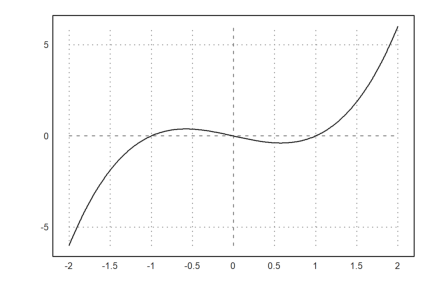
\includegraphics[keepaspectratio]{images/EMT4Plot2D - Naila Khalidatus Salwa-005.png}}
\caption{images/EMT4Plot2D\%20-\%20Naila\%20Khalidatus\%20Salwa-005.png}
\end{figure}

\textgreater a:=5.6; plot2d(``exp(-a*x\^{}2)/a''); insimg(30);

\begin{figure}
\centering
\pandocbounded{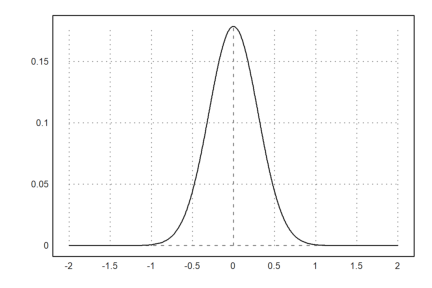
\includegraphics[keepaspectratio]{images/EMT4Plot2D - Naila Khalidatus Salwa-006.png}}
\caption{images/EMT4Plot2D\%20-\%20Naila\%20Khalidatus\%20Salwa-006.png}
\end{figure}

Plot di atas menampilkan gambar hasil plot setinggi 25 baris

Dari beberapa contoh sebelumnya Anda dapat melihat bahwa aslinya gambar plot menggunakan sumbu X dengan rentang nilai dari -2 sampai dengan 2. Untuk mengubah rentang nilai X dan Y, Anda dapat menambahkan nilai-nilai batas X (dan Y) di belakang ekspresi yang digambar.

Rentang plot diatur dengan parameter yang ditetapkan sebagai berikut

\begin{itemize}
\item
  a,b: x-range (default -2,2)
\item
  c,d: y-range (default: skala dengan nilai)
\item
  r: alternatifnya radius di sekitar pusat plot
\item
  cx,cy: koordinat pusat plot (default 0,0)
\end{itemize}

\textgreater plot2d(``x\^{}3-x'',-1,2): //plot dari fungsi x\^{}3-x dengan interval x dari -1 sampai 2

\begin{figure}
\centering
\pandocbounded{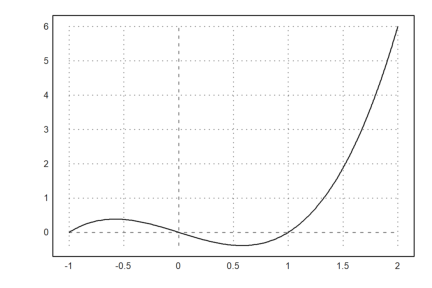
\includegraphics[keepaspectratio]{images/EMT4Plot2D - Naila Khalidatus Salwa-007.png}}
\caption{images/EMT4Plot2D\%20-\%20Naila\%20Khalidatus\%20Salwa-007.png}
\end{figure}

\textgreater plot2d(``sin(x)'',-2*pi,2*pi): // plot sin(x) pada interval {[}-2pi, 2pi{]}

\begin{figure}
\centering
\pandocbounded{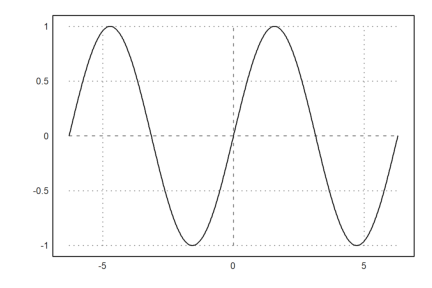
\includegraphics[keepaspectratio]{images/EMT4Plot2D - Naila Khalidatus Salwa-008.png}}
\caption{images/EMT4Plot2D\%20-\%20Naila\%20Khalidatus\%20Salwa-008.png}
\end{figure}

\textgreater plot2d(``cos(x)'',``sin(3*x)'',xmin=0,xmax=2pi):

\begin{figure}
\centering
\pandocbounded{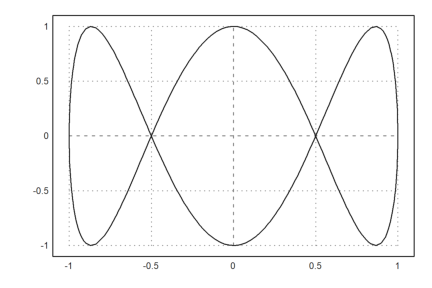
\includegraphics[keepaspectratio]{images/EMT4Plot2D - Naila Khalidatus Salwa-009.png}}
\caption{images/EMT4Plot2D\%20-\%20Naila\%20Khalidatus\%20Salwa-009.png}
\end{figure}

Alternatif untuk titik dua adalah perintah insimg(baris), yang menyisipkan plot yang menempati sejumlah baris teks tertentu.

Dalam opsi, plot dapat diatur agar muncul

\begin{itemize}
\item
  di jendela terpisah yang dapat diubah ukurannya,
\item
  di jendela notebook.
\end{itemize}

Lebih banyak gaya dapat dicapai dengan perintah plot tertentu.

Bagaimanapun, tekan tombol tabulator untuk melihat plotnya, jika tersembunyi.

Untuk membagi jendela menjadi beberapa plot, gunakan perintah figure(). Dalam contoh, kita memplot x\^{}1 hingga x\^{}4 menjadi 4 bagian jendela. gambar(0) mengatur ulang jendela default.

\textgreater reset;

\textgreater figure(2,2); \ldots{}\\
\textgreater{} for n=1 to 4; figure(n); plot2d(``x\^{}''+n); end; \ldots{}\\
\textgreater{} figure(0):

\begin{figure}
\centering
\pandocbounded{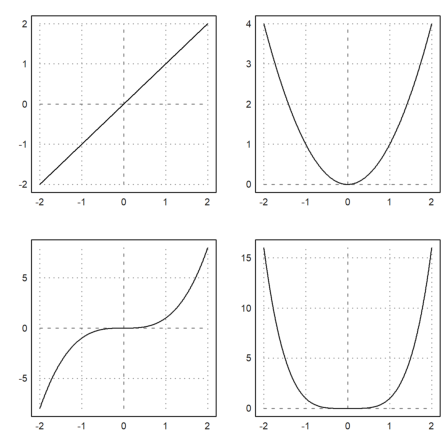
\includegraphics[keepaspectratio]{images/EMT4Plot2D - Naila Khalidatus Salwa-010.png}}
\caption{images/EMT4Plot2D\%20-\%20Naila\%20Khalidatus\%20Salwa-010.png}
\end{figure}

Di plot2d(), ada gaya alternatif yang tersedia dengan grid=x. Untuk gambaran umum, kami menampilkan berbagai gaya kisi dalam satu gambar (lihat di bawah untuk perintah figure()). Gaya grid=0 tidak disertakan. Ini tidak menunjukkan kisi dan bingkai.

\textgreater figure(3,3); \ldots{}\\
\textgreater{} for k=1:9; figure(k); plot2d(``x\^{}3-x'',-2,1,grid=k); end; \ldots{}\\
\textgreater{} figure(0):

\begin{figure}
\centering
\pandocbounded{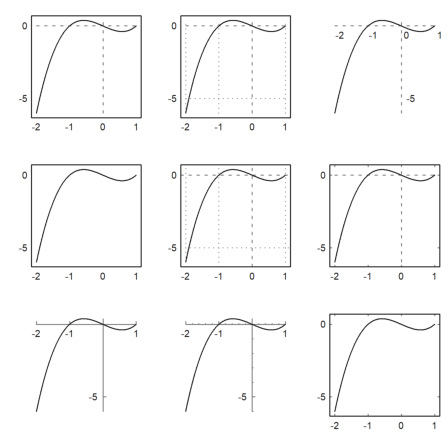
\includegraphics[keepaspectratio]{images/EMT4Plot2D - Naila Khalidatus Salwa-011.png}}
\caption{images/EMT4Plot2D\%20-\%20Naila\%20Khalidatus\%20Salwa-011.png}
\end{figure}

Jika argumen pada plot2d() adalah ekspresi yang diikuti oleh empat angka, angka-angka tersebut adalah rentang x dan y untuk plot tersebut.

Alternatifnya, a, b, c, d dapat ditentukan sebagai parameter yang ditetapkan sebagai a=\ldots{} dll.

Pada contoh berikut, kita mengubah gaya kisi, menambahkan label, dan menggunakan label vertikal untuk sumbu y.

\textgreater aspect(1.5); plot2d(``sin(x)'',0,2pi,-1.2,1.2,grid=3,xl=``x'',yl=``sin(x)''):

\begin{figure}
\centering
\pandocbounded{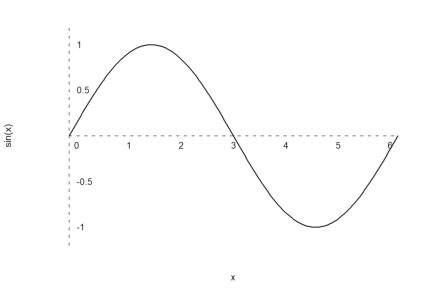
\includegraphics[keepaspectratio]{images/EMT4Plot2D - Naila Khalidatus Salwa-012.png}}
\caption{images/EMT4Plot2D\%20-\%20Naila\%20Khalidatus\%20Salwa-012.png}
\end{figure}

\textgreater plot2d(``sin(x)+cos(2*x)'',0,4pi):

\begin{figure}
\centering
\pandocbounded{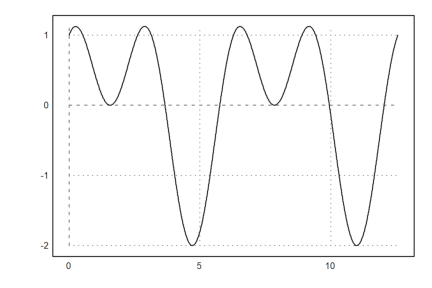
\includegraphics[keepaspectratio]{images/EMT4Plot2D - Naila Khalidatus Salwa-013.png}}
\caption{images/EMT4Plot2D\%20-\%20Naila\%20Khalidatus\%20Salwa-013.png}
\end{figure}

Gambar yang dihasilkan dengan memasukkan plot ke dalam jendela teks disimpan di direktori yang sama dengan notebook, secara default di subdirektori bernama ``images''. Mereka juga digunakan oleh ekspor HTML.

Anda cukup menandai gambar apa saja dan menyalinnya ke clipboard dengan Ctrl-C. Tentu saja, Anda juga dapat mengekspor grafik saat ini dengan fungsi di menu File.

Fungsi atau ekspresi di plot2d dievaluasi secara adaptif. Agar lebih cepat, nonaktifkan plot adaptif dengan \textless adaptive dan tentukan jumlah subinterval dengan n=\ldots{} Hal ini hanya diperlukan pada kasus yang jarang terjadi.

\textgreater plot2d(``sign(x)*exp(-x\^{}2)'',-1,1,\textless adaptive,n=10000):

\begin{figure}
\centering
\pandocbounded{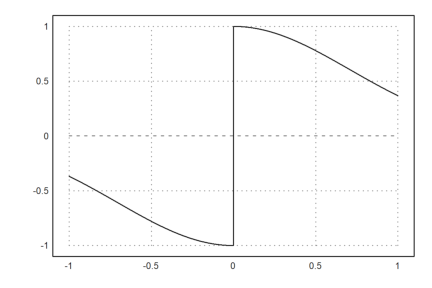
\includegraphics[keepaspectratio]{images/EMT4Plot2D - Naila Khalidatus Salwa-014.png}}
\caption{images/EMT4Plot2D\%20-\%20Naila\%20Khalidatus\%20Salwa-014.png}
\end{figure}

\textgreater plot2d(``x\^{}x'',r=1.2,cx=1,cy=1):

\begin{figure}
\centering
\pandocbounded{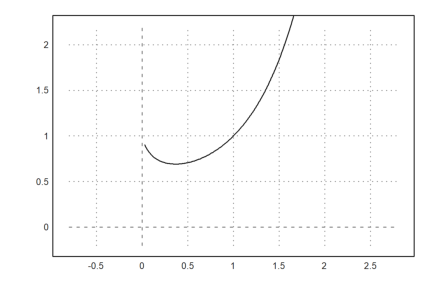
\includegraphics[keepaspectratio]{images/EMT4Plot2D - Naila Khalidatus Salwa-015.png}}
\caption{images/EMT4Plot2D\%20-\%20Naila\%20Khalidatus\%20Salwa-015.png}
\end{figure}

Perhatikan bahwa x\^{}x tidak ditentukan untuk x\textless=0. Fungsi plot2d menangkap kesalahan ini, dan mulai membuat plot segera setelah fungsinya ditentukan. Ini berfungsi untuk semua fungsi yang mengembalikan NAN di luar jangkauan definisinya.

\textgreater plot2d(``log(x)'',-0.1,2):

\begin{figure}
\centering
\pandocbounded{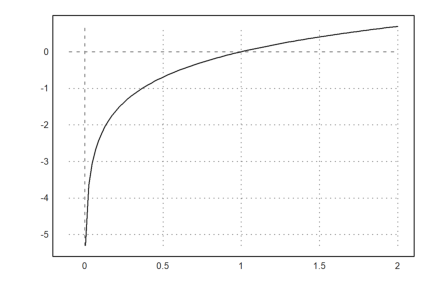
\includegraphics[keepaspectratio]{images/EMT4Plot2D - Naila Khalidatus Salwa-016.png}}
\caption{images/EMT4Plot2D\%20-\%20Naila\%20Khalidatus\%20Salwa-016.png}
\end{figure}

Parameter square=true (atau \textgreater square) memilih rentang y secara otomatis sehingga hasilnya adalah jendela plot persegi. Perhatikan bahwa secara default, Euler menggunakan spasi persegi di dalam jendela plot.

\textgreater plot2d(``x\^{}3-x'',\textgreater square):

\begin{figure}
\centering
\pandocbounded{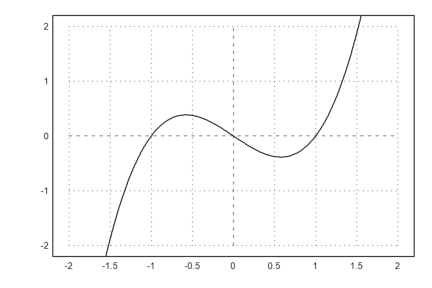
\includegraphics[keepaspectratio]{images/EMT4Plot2D - Naila Khalidatus Salwa-017.png}}
\caption{images/EMT4Plot2D\%20-\%20Naila\%20Khalidatus\%20Salwa-017.png}
\end{figure}

\textgreater plot2d(`'integrate(``sin(x)*exp(-x\^{}2)'',0,x)'\,',0,2): // plot integral

\begin{figure}
\centering
\pandocbounded{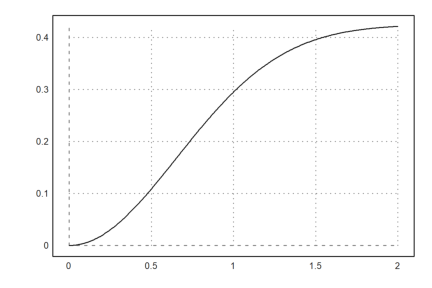
\includegraphics[keepaspectratio]{images/EMT4Plot2D - Naila Khalidatus Salwa-018.png}}
\caption{images/EMT4Plot2D\%20-\%20Naila\%20Khalidatus\%20Salwa-018.png}
\end{figure}

Jika Anda memerlukan lebih banyak ruang untuk label y, panggil shrinkwindow() dengan parameter lebih kecil, atau tetapkan nilai positif untuk ``smaller'' di plot2d().

\textgreater plot2d(``gamma(x)'',1,10,yl=``y-values'',smaller=6,\textless vertical):

\begin{figure}
\centering
\pandocbounded{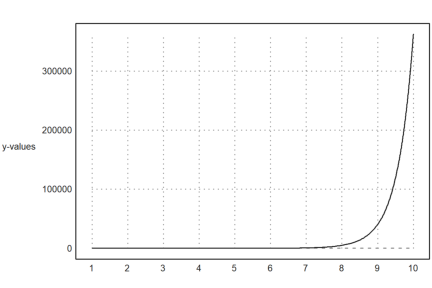
\includegraphics[keepaspectratio]{images/EMT4Plot2D - Naila Khalidatus Salwa-019.png}}
\caption{images/EMT4Plot2D\%20-\%20Naila\%20Khalidatus\%20Salwa-019.png}
\end{figure}

Ekspresi simbolik juga dapat digunakan karena disimpan sebagai ekspresi string sederhana.

\textgreater x=linspace(0,2pi,1000); plot2d(sin(5x),cos(7x)):

\begin{figure}
\centering
\pandocbounded{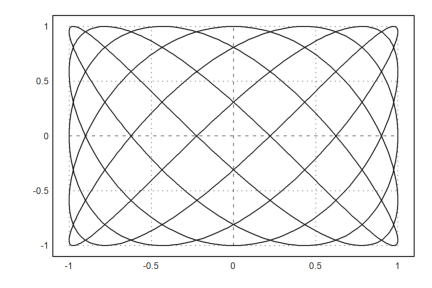
\includegraphics[keepaspectratio]{images/EMT4Plot2D - Naila Khalidatus Salwa-020.png}}
\caption{images/EMT4Plot2D\%20-\%20Naila\%20Khalidatus\%20Salwa-020.png}
\end{figure}

\textgreater a:=5.6; expr \&= exp(-a*x\^{}2)/a; // mendefinisikan ekspresi

\textgreater plot2d(expr,-2,2): // plot dari -2 sampai 2

\begin{figure}
\centering
\pandocbounded{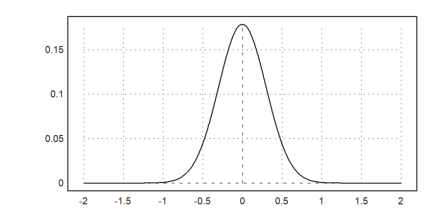
\includegraphics[keepaspectratio]{images/EMT4Plot2D - Naila Khalidatus Salwa-021.png}}
\caption{images/EMT4Plot2D\%20-\%20Naila\%20Khalidatus\%20Salwa-021.png}
\end{figure}

\textgreater plot2d(expr,r=1,thickness=3): // plot di sekitar persegi (0,0)

\begin{figure}
\centering
\pandocbounded{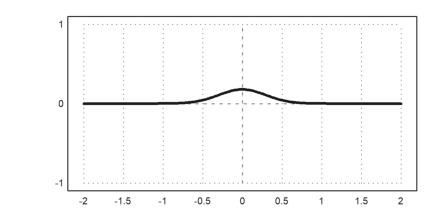
\includegraphics[keepaspectratio]{images/EMT4Plot2D - Naila Khalidatus Salwa-022.png}}
\caption{images/EMT4Plot2D\%20-\%20Naila\%20Khalidatus\%20Salwa-022.png}
\end{figure}

\textgreater plot2d(\&diff(expr,x),\textgreater add,style=``--'',color=red): // menambahkan plot lainnya

\begin{figure}
\centering
\pandocbounded{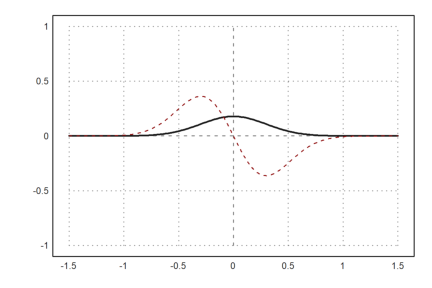
\includegraphics[keepaspectratio]{images/EMT4Plot2D - Naila Khalidatus Salwa-023.png}}
\caption{images/EMT4Plot2D\%20-\%20Naila\%20Khalidatus\%20Salwa-023.png}
\end{figure}

\textgreater plot2d(\&diff(expr,x,2),a=-2,b=2,c=-2,d=1): // plot in rectangle

\begin{figure}
\centering
\pandocbounded{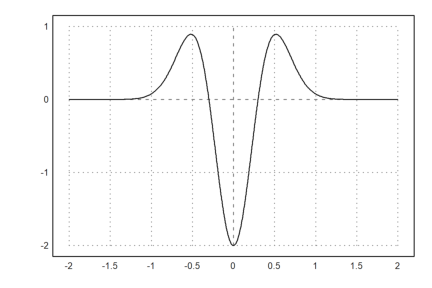
\includegraphics[keepaspectratio]{images/EMT4Plot2D - Naila Khalidatus Salwa-024.png}}
\caption{images/EMT4Plot2D\%20-\%20Naila\%20Khalidatus\%20Salwa-024.png}
\end{figure}

\textgreater plot2d(\&diff(expr,x),a=-2,b=2,\textgreater square): // menetapkan plot square

\begin{figure}
\centering
\pandocbounded{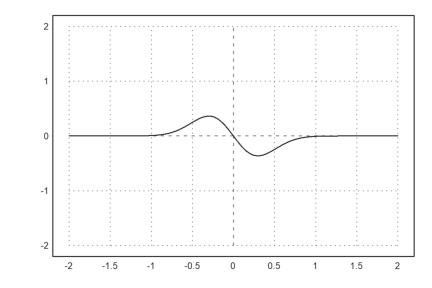
\includegraphics[keepaspectratio]{images/EMT4Plot2D - Naila Khalidatus Salwa-025.png}}
\caption{images/EMT4Plot2D\%20-\%20Naila\%20Khalidatus\%20Salwa-025.png}
\end{figure}

\textgreater plot2d(``x\^{}2'',0,1,steps=1,color=red,n=10):

\begin{figure}
\centering
\pandocbounded{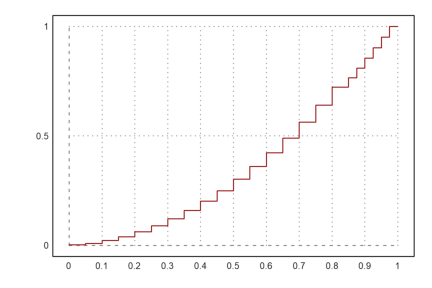
\includegraphics[keepaspectratio]{images/EMT4Plot2D - Naila Khalidatus Salwa-026.png}}
\caption{images/EMT4Plot2D\%20-\%20Naila\%20Khalidatus\%20Salwa-026.png}
\end{figure}

\textgreater plot2d(``x\^{}2'',\textgreater add,steps=2,color=blue,n=10):

\begin{figure}
\centering
\pandocbounded{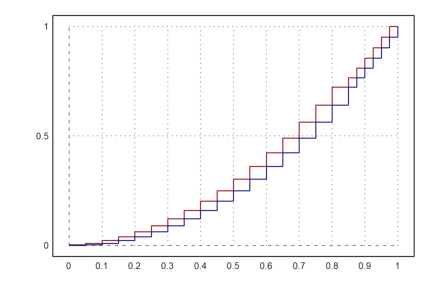
\includegraphics[keepaspectratio]{images/EMT4Plot2D - Naila Khalidatus Salwa-027.png}}
\caption{images/EMT4Plot2D\%20-\%20Naila\%20Khalidatus\%20Salwa-027.png}
\end{figure}

\chapter{Fungsi dalam satu Parameter}\label{fungsi-dalam-satu-parameter}

Fungsi plot yang paling penting untuk plot planar adalah plot2d(). Fungsi ini diimplementasikan dalam bahasa Euler di file ``plot.e'', yang dimuat di awal program.

Berikut beberapa contoh penggunaan suatu fungsi. Seperti biasa di EMT, fungsi yang berfungsi untuk fungsi atau ekspresi lain, Anda bisa meneruskan parameter tambahan (selain x) yang bukan variabel global ke fungsi dengan parameter titik koma atau dengan kumpulan panggilan.

\textgreater function f(x,a) := x\textsuperscript{2/a+a*x}2-x; // mendefinisikan fungsi a

\textgreater a=0.3; plot2d(``f'',0,1;a): // plot dengan a=0.3

\begin{figure}
\centering
\pandocbounded{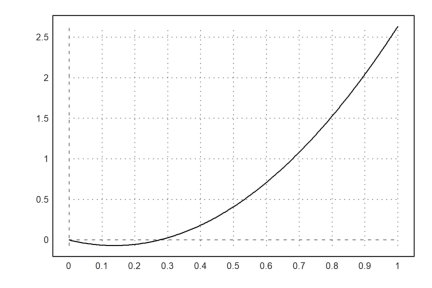
\includegraphics[keepaspectratio]{images/EMT4Plot2D - Naila Khalidatus Salwa-028.png}}
\caption{images/EMT4Plot2D\%20-\%20Naila\%20Khalidatus\%20Salwa-028.png}
\end{figure}

\textgreater plot2d(``f'',0,1;0.4): // plot dengan a=0.4

\begin{figure}
\centering
\pandocbounded{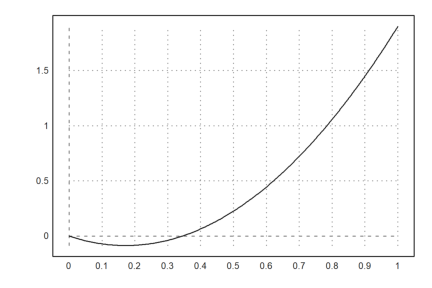
\includegraphics[keepaspectratio]{images/EMT4Plot2D - Naila Khalidatus Salwa-029.png}}
\caption{images/EMT4Plot2D\%20-\%20Naila\%20Khalidatus\%20Salwa-029.png}
\end{figure}

\textgreater plot2d(\{\{``f'',0.2\}\},0,1): // plot dengan a=0.2

\begin{figure}
\centering
\pandocbounded{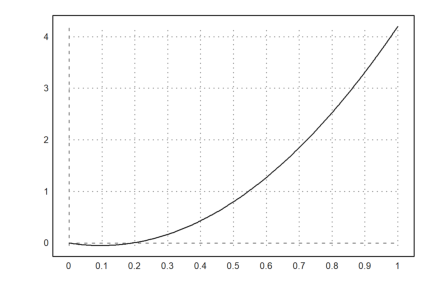
\includegraphics[keepaspectratio]{images/EMT4Plot2D - Naila Khalidatus Salwa-030.png}}
\caption{images/EMT4Plot2D\%20-\%20Naila\%20Khalidatus\%20Salwa-030.png}
\end{figure}

\textgreater plot2d(\{\{``f(x,b)'',b=0.1\}\},0,1): // plot dengan a=0.1

\begin{figure}
\centering
\pandocbounded{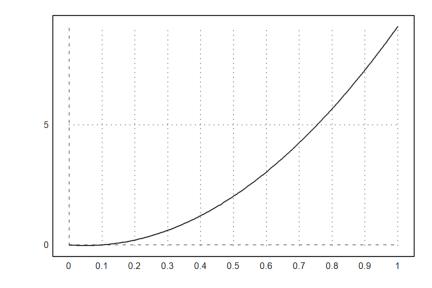
\includegraphics[keepaspectratio]{images/EMT4Plot2D - Naila Khalidatus Salwa-031.png}}
\caption{images/EMT4Plot2D\%20-\%20Naila\%20Khalidatus\%20Salwa-031.png}
\end{figure}

\textgreater function f(x) := x\^{}3-x; \ldots{}\\
\textgreater{} plot2d(``f'',r=1):

\begin{figure}
\centering
\pandocbounded{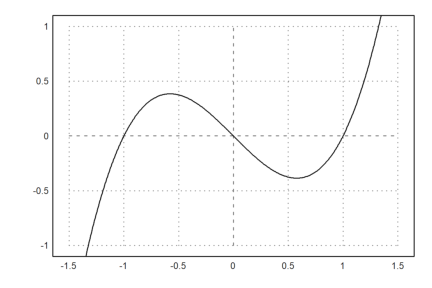
\includegraphics[keepaspectratio]{images/EMT4Plot2D - Naila Khalidatus Salwa-032.png}}
\caption{images/EMT4Plot2D\%20-\%20Naila\%20Khalidatus\%20Salwa-032.png}
\end{figure}

Berikut ini ringkasan fungsi yang diterima

\begin{itemize}
\item
  ekspresi atau ekspresi simbolik di x
\item
  fungsi atau fungsi simbolik dengan nama ``f''
\item
  fungsi simbolik hanya dengan nama f
\end{itemize}

Fungsi plot2d() juga menerima fungsi simbolik. Untuk fungsi simbolik, namanya saja yang berfungsi.

\textgreater function f(x) \&= diff(x\^{}x,x)

\begin{verbatim}
                            x
                           x  (log(x) + 1)
\end{verbatim}

\textgreater plot2d(f,0,2):

\begin{figure}
\centering
\pandocbounded{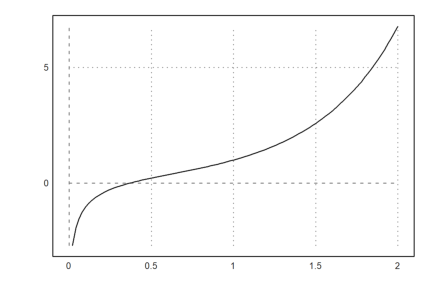
\includegraphics[keepaspectratio]{images/EMT4Plot2D - Naila Khalidatus Salwa-033.png}}
\caption{images/EMT4Plot2D\%20-\%20Naila\%20Khalidatus\%20Salwa-033.png}
\end{figure}

Tentu saja, untuk ekspresi atau ekspresi simbolik, nama variabel sudah cukup untuk memplotnya.

\textgreater expr \&= sin(x)*exp(-x)

\begin{verbatim}
                              - x
                             E    sin(x)
\end{verbatim}

\textgreater plot2d(expr,0,3pi):

\begin{figure}
\centering
\pandocbounded{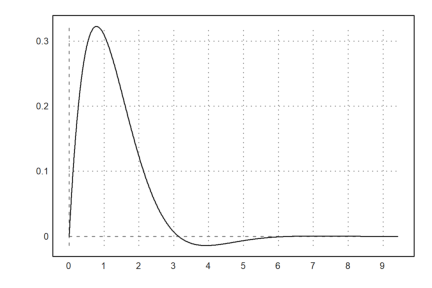
\includegraphics[keepaspectratio]{images/EMT4Plot2D - Naila Khalidatus Salwa-034.png}}
\caption{images/EMT4Plot2D\%20-\%20Naila\%20Khalidatus\%20Salwa-034.png}
\end{figure}

\textgreater function f(x) \&= x\^{}x;

\textgreater plot2d(f,r=1,cx=1,cy=1,color=blue,thickness=2);

\textgreater plot2d(\&diff(f(x),x),\textgreater add,color=red,style=``-.-''):

\begin{figure}
\centering
\pandocbounded{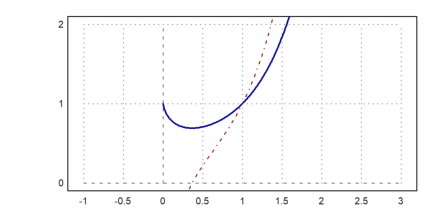
\includegraphics[keepaspectratio]{images/EMT4Plot2D - Naila Khalidatus Salwa-035.png}}
\caption{images/EMT4Plot2D\%20-\%20Naila\%20Khalidatus\%20Salwa-035.png}
\end{figure}

Ada berbagai pilihan untuk gaya garis

\begin{itemize}
\item
  style=``\ldots{}''. Memilih di antara ``-'', ``--'', ``-.'', ``.'', ``.-.'', ``-.-''.
\item
  warna: Lihat di bawah untuk warna.
\item
  ketebalan: Defaultnya adalah 1.
\end{itemize}

Warna dapat dipilih sebagai salah satu warna default, atau sebagai warna RGB.

\begin{itemize}
\item
  0..15: indeks warna default.
\item
  warna yang tersedia: white, black, red, green, blue, cyan, olive,
\item
  lightgray, gray, darkgray, orange, lightgreen, turquoise, lightblue,
\item
  lightorange, yellow
\item
  rgb(red,green,blue): parameternya real di {[}0,1{]}.
\end{itemize}

\textgreater plot2d(``exp(-x\^{}2)'',r=2,color=red,thickness=3,style=``--''):

\begin{figure}
\centering
\pandocbounded{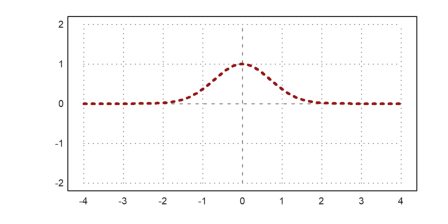
\includegraphics[keepaspectratio]{images/EMT4Plot2D - Naila Khalidatus Salwa-036.png}}
\caption{images/EMT4Plot2D\%20-\%20Naila\%20Khalidatus\%20Salwa-036.png}
\end{figure}

Berikut adalah tampilan warna EMT yang telah ditentukan sebelumnya.

\textgreater aspect(2); columnsplot(ones(1,16),lab=0:15,grid=0,color=0:15)://menampilkan warna-warna yang tersedia

\begin{figure}
\centering
\pandocbounded{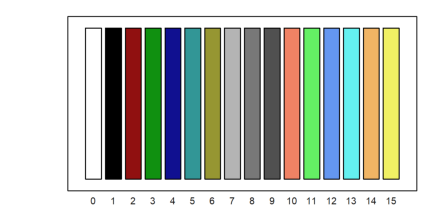
\includegraphics[keepaspectratio]{images/EMT4Plot2D - Naila Khalidatus Salwa-037.png}}
\caption{images/EMT4Plot2D\%20-\%20Naila\%20Khalidatus\%20Salwa-037.png}
\end{figure}

Tapi kita bisa menggunakan warna apa saja.

\textgreater columnsplot(ones(1,16),grid=0,color=rgb(0,0,linspace(0,1,15))):

\begin{figure}
\centering
\pandocbounded{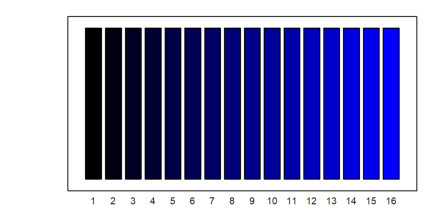
\includegraphics[keepaspectratio]{images/EMT4Plot2D - Naila Khalidatus Salwa-038.png}}
\caption{images/EMT4Plot2D\%20-\%20Naila\%20Khalidatus\%20Salwa-038.png}
\end{figure}

\chapter{Menggambar Beberapa Kurva pada bidang koordinat yang sama}\label{menggambar-beberapa-kurva-pada-bidang-koordinat-yang-sama}

Menggambar plot lebih dari satu fungsi (multiple function) ke dalam satu jendela dapat dilakukan dengan berbagai cara. Salah satu metodenya adalah menggunakan \textgreater add untuk beberapa panggilan ke plot2d secara keseluruhan, kecuali panggilan pertama. Kami telah menggunakan fitur ini pada contoh di atas.

\textgreater aspect(); plot2d(``cos(x)'',r=2,grid=6); plot2d(``x'',style=``.'',\textgreater add):

\begin{figure}
\centering
\pandocbounded{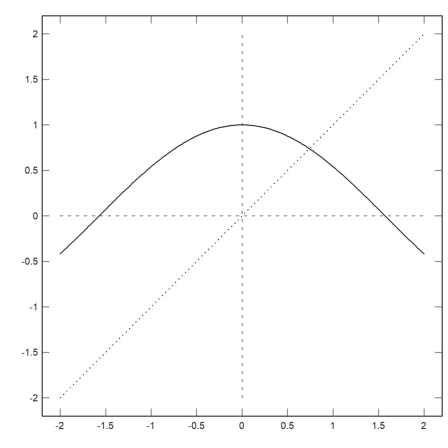
\includegraphics[keepaspectratio]{images/EMT4Plot2D - Naila Khalidatus Salwa-039.png}}
\caption{images/EMT4Plot2D\%20-\%20Naila\%20Khalidatus\%20Salwa-039.png}
\end{figure}

\textgreater aspect(1.5); plot2d(``sin(x)'',0,2pi); plot2d(``cos(x)'',color=blue,style=``--'',\textgreater add):

\begin{figure}
\centering
\pandocbounded{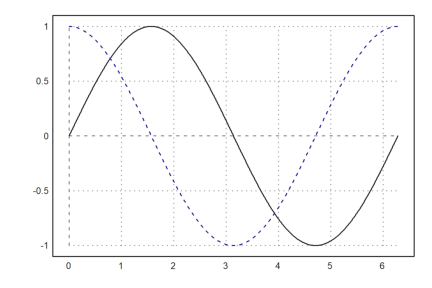
\includegraphics[keepaspectratio]{images/EMT4Plot2D - Naila Khalidatus Salwa-040.png}}
\caption{images/EMT4Plot2D\%20-\%20Naila\%20Khalidatus\%20Salwa-040.png}
\end{figure}

Salah satu kegunaan \textgreater add adalah untuk menambahkan titik pada kurva.

\textgreater plot2d(``sin(x)'',0,pi); plot2d(2,sin(2),\textgreater points,\textgreater add):

\begin{figure}
\centering
\pandocbounded{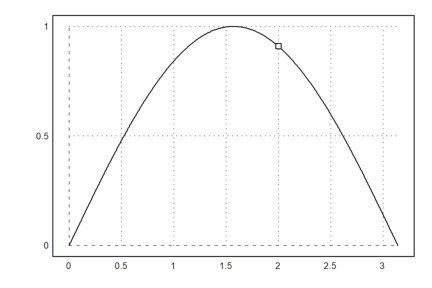
\includegraphics[keepaspectratio]{images/EMT4Plot2D - Naila Khalidatus Salwa-041.png}}
\caption{images/EMT4Plot2D\%20-\%20Naila\%20Khalidatus\%20Salwa-041.png}
\end{figure}

Kita tambahkan titik perpotongan dengan label (pada posisi ``cl'' untuk kiri tengah), dan masukkan hasilnya ke dalam buku catatan. Kami juga menambahkan judul pada plot.

\textgreater plot2d({[}``cos(x)'',``x''{]},r=1.1,cx=0.5,cy=0.5, \ldots{}\\
\textgreater{} color={[}black,blue{]},style={[}``-'',``.''{]}, \ldots{}\\
\textgreater{} grid=1);

\textgreater x0=solve(``cos(x)-x'',1); \ldots{}\\
\textgreater{} plot2d(x0,x0,\textgreater points,\textgreater add,title=``Intersection Demo''); \ldots{}\\
\textgreater{} label(``cos(x) = x'',x0,x0,pos=``cl'',offset=20):

\begin{figure}
\centering
\pandocbounded{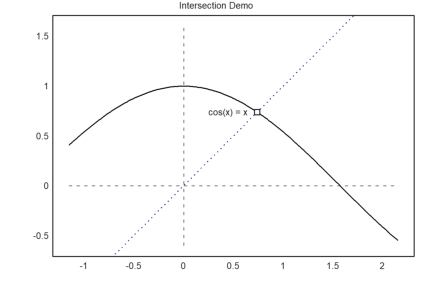
\includegraphics[keepaspectratio]{images/EMT4Plot2D - Naila Khalidatus Salwa-042.png}}
\caption{images/EMT4Plot2D\%20-\%20Naila\%20Khalidatus\%20Salwa-042.png}
\end{figure}

Dalam demo berikut, kita membuat plot fungsi sin(x)=sin(x)/x dan ekspansi Taylor ke-8 dan ke-16. Kami menghitung perluasan ini menggunakan Maxima melalui ekspresi simbolik.

Plot ini dilakukan dalam perintah multi-baris berikut dengan tiga panggilan ke plot2d(). Yang kedua dan ketiga memiliki kumpulan tanda \textgreater add, yang membuat plot menggunakan rentang sebelumnya.

Kami menambahkan kotak label yang menjelaskan fungsinya.

\textgreater\$taylor(sin(x)/x,x,0,4)

\[\frac{x^4}{120}-\frac{x^2}{6}+1\]\textgreater{} plot2d(``sinc(x)'',0,4pi,color=green,thickness=2); \ldots{}\\
\textgreater{} plot2d(\&taylor(sin(x)/x,x,0,8),\textgreater add,color=blue,style=``--''); \ldots{}\\
\textgreater{} plot2d(\&taylor(sin(x)/x,x,0,16),\textgreater add,color=red,style=``-.-''); \ldots{}\\
\textgreater{} labelbox({[}``sinc'',``T8'',``T16''{]},styles={[}``-'',``--'',``-.-''{]}, \ldots{}\\
\textgreater{} colors={[}black,blue,red{]}):

\begin{figure}
\centering
\pandocbounded{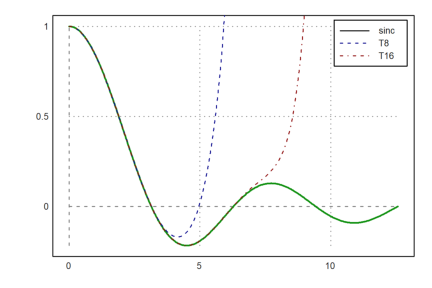
\includegraphics[keepaspectratio]{images/EMT4Plot2D - Naila Khalidatus Salwa-044.png}}
\caption{images/EMT4Plot2D\%20-\%20Naila\%20Khalidatus\%20Salwa-044.png}
\end{figure}

Dalam contoh berikut, kami menghasilkan Polinomial Bernstein.

\[B_i(x) = \binom{n}{i} x^i (1-x)^{n-i}\]\textgreater plot2d(``(1-x)\^{}10'',0,1); // plot fungsi pertama

\textgreater insimg;

\begin{figure}
\centering
\pandocbounded{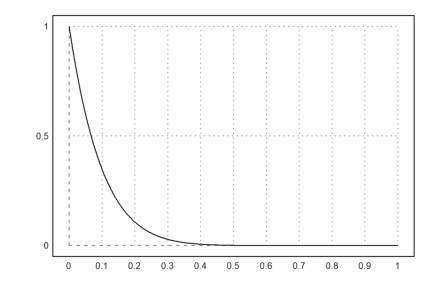
\includegraphics[keepaspectratio]{images/EMT4Plot2D - Naila Khalidatus Salwa-046.png}}
\caption{images/EMT4Plot2D\%20-\%20Naila\%20Khalidatus\%20Salwa-046.png}
\end{figure}

\textgreater for i=1 to 10; plot2d(``bin(10,i)*x\textsuperscript{i*(1-x)}(10-i)'',\textgreater add); end;

\textgreater insimg;

\begin{figure}
\centering
\pandocbounded{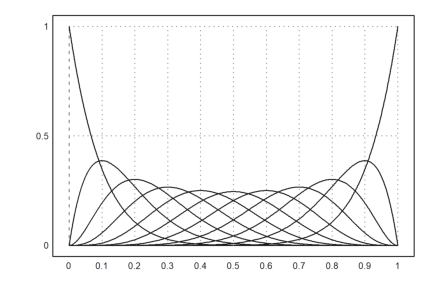
\includegraphics[keepaspectratio]{images/EMT4Plot2D - Naila Khalidatus Salwa-047.png}}
\caption{images/EMT4Plot2D\%20-\%20Naila\%20Khalidatus\%20Salwa-047.png}
\end{figure}

Cara kedua adalah dengan menggunakan pasangan matriks bernilai x dan matriks bernilai y yang berukuran sama.

Kami menghasilkan matriks nilai dengan satu Polinomial Bernstein di setiap baris. Untuk ini, kita cukup menggunakan vektor kolom i. Lihat pendahuluan tentang bahasa matriks untuk mempelajari lebih detail.

\textgreater x=linspace(0,1,500);

\textgreater n=10; k=(0:n)'; // n adalah vektor baris, k adalah vektor kolom

\textgreater y=bin(n,k)*x\textsuperscript{k*(1-x)}(n-k); // y adalah sebuah matriks

\textgreater plot2d(x,y):

\begin{figure}
\centering
\pandocbounded{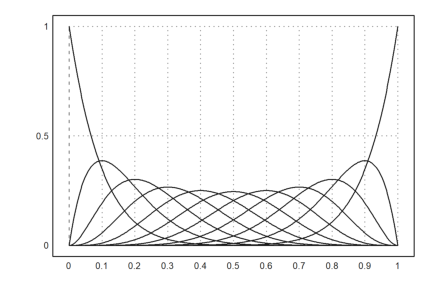
\includegraphics[keepaspectratio]{images/EMT4Plot2D - Naila Khalidatus Salwa-048.png}}
\caption{images/EMT4Plot2D\%20-\%20Naila\%20Khalidatus\%20Salwa-048.png}
\end{figure}

Perhatikan bahwa parameter warna dapat berupa vektor. Kemudian setiap warna digunakan untuk setiap baris matriks.

\textgreater x=linspace(0,1,200); y=x\^{}(1:10)'; plot2d(x,y,color=1:10):

\begin{figure}
\centering
\pandocbounded{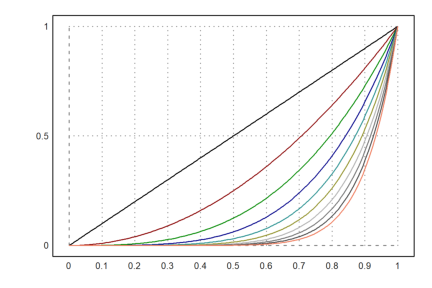
\includegraphics[keepaspectratio]{images/EMT4Plot2D - Naila Khalidatus Salwa-049.png}}
\caption{images/EMT4Plot2D\%20-\%20Naila\%20Khalidatus\%20Salwa-049.png}
\end{figure}

Metode lain adalah menggunakan vektor ekspresi (string). Anda kemudian dapat menggunakan susunan warna, susunan gaya, dan susunan ketebalan dengan panjang yang sama.

\textgreater plot2d({[}``sin(x)'',``cos(x)''{]},0,2pi,color=4:5):

\begin{figure}
\centering
\pandocbounded{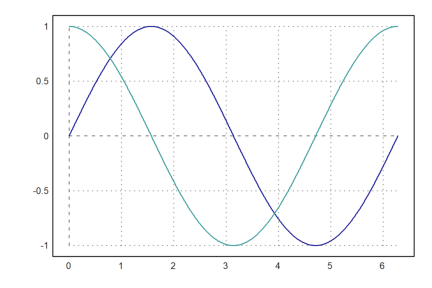
\includegraphics[keepaspectratio]{images/EMT4Plot2D - Naila Khalidatus Salwa-050.png}}
\caption{images/EMT4Plot2D\%20-\%20Naila\%20Khalidatus\%20Salwa-050.png}
\end{figure}

\textgreater plot2d({[}``sin(x)'',``cos(x)''{]},0,2pi): // plot vector dari ekspresi

\begin{figure}
\centering
\pandocbounded{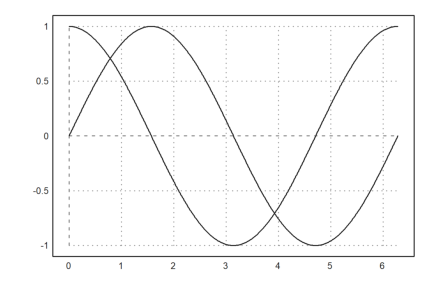
\includegraphics[keepaspectratio]{images/EMT4Plot2D - Naila Khalidatus Salwa-051.png}}
\caption{images/EMT4Plot2D\%20-\%20Naila\%20Khalidatus\%20Salwa-051.png}
\end{figure}

Kita bisa mendapatkan vektor seperti itu dari Maxima menggunakan makelist() dan mxm2str().

\textgreater v \&= makelist(binomial(10,i)*x\textsuperscript{i*(1-x)}(10-i),i,0,10) // membuat list

\begin{verbatim}
               10            9              8  2             7  3
       [(1 - x)  , 10 (1 - x)  x, 45 (1 - x)  x , 120 (1 - x)  x , 
           6  4             5  5             4  6             3  7
210 (1 - x)  x , 252 (1 - x)  x , 210 (1 - x)  x , 120 (1 - x)  x , 
          2  8              9   10
45 (1 - x)  x , 10 (1 - x) x , x  ]
\end{verbatim}

\textgreater mxm2str(v) // mendapatkan sebuah vektor string dari vektor simbolik

\begin{verbatim}
(1-x)^10
10*(1-x)^9*x
45*(1-x)^8*x^2
120*(1-x)^7*x^3
210*(1-x)^6*x^4
252*(1-x)^5*x^5
210*(1-x)^4*x^6
120*(1-x)^3*x^7
45*(1-x)^2*x^8
10*(1-x)*x^9
x^10
\end{verbatim}

\textgreater plot2d(mxm2str(v),0,1): // plot fungsi

\begin{figure}
\centering
\pandocbounded{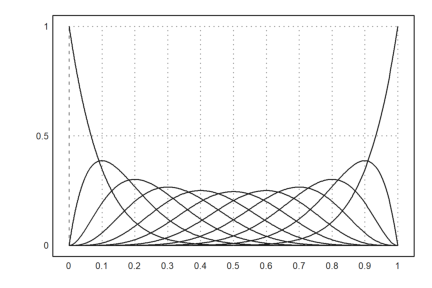
\includegraphics[keepaspectratio]{images/EMT4Plot2D - Naila Khalidatus Salwa-052.png}}
\caption{images/EMT4Plot2D\%20-\%20Naila\%20Khalidatus\%20Salwa-052.png}
\end{figure}

Alternatif lain adalah dengan menggunakan bahasa matriks Euler.

Jika suatu ekspresi menghasilkan matriks fungsi, dengan satu fungsi di setiap baris, semua fungsi tersebut akan diplot ke dalam satu plot.

Untuk ini, gunakan vektor parameter dalam bentuk vektor kolom. Jika array warna ditambahkan maka akan digunakan untuk setiap baris plot.

\textgreater n=(1:10)'; plot2d(``x\^{}n'',0,1,color=1:10)://membuat plot dengan setiap nilai n warna nya berbeda

\begin{figure}
\centering
\pandocbounded{\includegraphics[keepaspectratio]{images/EMT4Plot2D - Naila Khalidatus Salwa-053.png}}
\caption{images/EMT4Plot2D\%20-\%20Naila\%20Khalidatus\%20Salwa-053.png}
\end{figure}

Ekspresi dan fungsi satu baris dapat melihat variabel global.

Jika Anda tidak dapat menggunakan variabel global, Anda perlu menggunakan fungsi dengan parameter tambahan, dan meneruskan parameter ini sebagai parameter titik koma.

Berhati-hatilah, untuk meletakkan semua parameter yang ditetapkan di akhir perintah plot2d. Dalam contoh ini kita meneruskan a=5 ke fungsi f, yang kita plot dari -10 hingga 10.

\textgreater function f(x,a) := 1/a*exp(-x\^{}2/a); \ldots{}\\
\textgreater{} plot2d(``f'',-10,10;5,thickness=2,title=``a=5''):

\begin{figure}
\centering
\pandocbounded{\includegraphics[keepaspectratio]{images/EMT4Plot2D - Naila Khalidatus Salwa-054.png}}
\caption{images/EMT4Plot2D\%20-\%20Naila\%20Khalidatus\%20Salwa-054.png}
\end{figure}

Alternatifnya, gunakan koleksi dengan nama fungsi dan semua parameter tambahan. Daftar khusus ini disebut kumpulan panggilan, dan ini adalah cara yang lebih disukai untuk meneruskan argumen ke suatu fungsi yang kemudian diteruskan sebagai argumen ke fungsi lain.

Pada contoh berikut, kita menggunakan loop untuk memplot beberapa fungsi (lihat tutorial tentang pemrograman loop).

\textgreater plot2d(\{\{``f'',1\}\},-10,10); \ldots{}\\
\textgreater{} for a=2:10; plot2d(\{\{``f'',a\}\},\textgreater add); end:

\begin{figure}
\centering
\pandocbounded{\includegraphics[keepaspectratio]{images/EMT4Plot2D - Naila Khalidatus Salwa-055.png}}
\caption{images/EMT4Plot2D\%20-\%20Naila\%20Khalidatus\%20Salwa-055.png}
\end{figure}

Kita dapat mencapai hasil yang sama dengan cara berikut menggunakan bahasa matriks EMT. Setiap baris matriks f(x,a) merupakan satu fungsi. Selain itu, kita dapat mengatur warna untuk setiap baris matriks. Klik dua kali pada fungsi getspectral() untuk penjelasannya.

\textgreater x=-10:0.01:10; a=(1:10)'; plot2d(x,f(x,a),color=getspectral(a/10)):

\begin{figure}
\centering
\pandocbounded{\includegraphics[keepaspectratio]{images/EMT4Plot2D - Naila Khalidatus Salwa-056.png}}
\caption{images/EMT4Plot2D\%20-\%20Naila\%20Khalidatus\%20Salwa-056.png}
\end{figure}

\textgreater{}

\chapter{Soal latihan tambahan}\label{soal-latihan-tambahan}

\begin{enumerate}
\def\labelenumi{\arabic{enumi}.}
\tightlist
\item
  Sketsakan grafik fungsi berikut di interval 1:10
\end{enumerate}

\[g(x)= \sqrt{(x+3)} +1\]\textgreater{} function g(x) := sqrt(x+3) + 1;\ldots{}\\
\textgreater{} for x=1:10; plot2d (``g'', 1, 10, title=``Grafik g(x)''); end:

\begin{figure}
\centering
\pandocbounded{\includegraphics[keepaspectratio]{images/EMT4Plot2D - Naila Khalidatus Salwa-058.png}}
\caption{images/EMT4Plot2D\%20-\%20Naila\%20Khalidatus\%20Salwa-058.png}
\end{figure}

\begin{enumerate}
\def\labelenumi{\arabic{enumi}.}
\setcounter{enumi}{1}
\tightlist
\item
  Carilah grafik dari fungsi berikut pada interval {[}-pi,2pi{]}
\end{enumerate}

\[y = sin  ({t - \frac{t}{4}})\]\textgreater function y(t) := sin (t-(t/4));\ldots{}\\
\textgreater{} plot2d (``y'', -pi, 2pi, color=green, title=``Grafik y(t)''):

\begin{figure}
\centering
\pandocbounded{\includegraphics[keepaspectratio]{images/EMT4Plot2D - Naila Khalidatus Salwa-060.png}}
\caption{images/EMT4Plot2D\%20-\%20Naila\%20Khalidatus\%20Salwa-060.png}
\end{figure}

\section{Label Teks}\label{label-teks}

Dekorasi sederhana pun bisa

\begin{itemize}
\item
  judul dengan judul = ``\ldots{}''
\item
  label x dan y dengan xl=``\ldots{}'', yl=``\ldots{}''
\item
  label teks lain dengan label(``\ldots{}'',x,y)
\end{itemize}

Perintah label akan memplot ke plot saat ini pada koordinat plot (x,y). Hal ini memerlukan argumen posisional.

\textgreater plot2d(``x\textsuperscript{3-x'',-1,2,title=''y=x}3-x'',yl=``y'',xl=``x''):

\begin{figure}
\centering
\pandocbounded{\includegraphics[keepaspectratio]{images/EMT4Plot2D - Naila Khalidatus Salwa-061.png}}
\caption{images/EMT4Plot2D\%20-\%20Naila\%20Khalidatus\%20Salwa-061.png}
\end{figure}

\textgreater expr := ``log(x)/x''; \ldots{}\\
\textgreater{} plot2d(expr,0.5,5,title=``y=''+expr,xl=``x'',yl=``y''); \ldots{}\\
\textgreater{} label(``(1,0)'',1,0); label(``Max'',E,expr(E),pos=``lc''):

\begin{figure}
\centering
\pandocbounded{\includegraphics[keepaspectratio]{images/EMT4Plot2D - Naila Khalidatus Salwa-062.png}}
\caption{images/EMT4Plot2D\%20-\%20Naila\%20Khalidatus\%20Salwa-062.png}
\end{figure}

Ada juga fungsi labelbox(), yang dapat menampilkan fungsi dan teks. Dibutuhkan vektor string dan warna, satu item untuk setiap fungsi.

\textgreater function f(x) \&= x\textsuperscript{2*exp(-x}2); \ldots{}\\
\textgreater{} plot2d(\&f(x),a=-3,b=3,c=-1,d=1); \ldots{}\\
\textgreater{} plot2d(\&diff(f(x),x),\textgreater add,color=blue,style=``--''); \ldots{}\\
\textgreater{} labelbox({[}``function'',``derivative''{]},styles={[}``-'',``--''{]}, \ldots{}\\
\textgreater{} colors={[}black,blue{]},w=0.4):

\begin{figure}
\centering
\pandocbounded{\includegraphics[keepaspectratio]{images/EMT4Plot2D - Naila Khalidatus Salwa-063.png}}
\caption{images/EMT4Plot2D\%20-\%20Naila\%20Khalidatus\%20Salwa-063.png}
\end{figure}

Kotak ini berada di kanan atas secara default, tetapi \textgreater kiri berlabuh di kiri atas. Anda dapat memindahkannya ke tempat mana pun yang Anda suka. Posisi jangkar berada di pojok kanan atas kotak, dan angkanya merupakan pecahan dari ukuran jendela grafis. Lebarnya otomatis.

Untuk plot titik, kotak label juga berfungsi. Tambahkan parameter \textgreater points, atau vektor bendera, satu untuk setiap label.

Pada contoh berikut, hanya ada satu fungsi. Jadi kita bisa menggunakan string sebagai pengganti vektor string. Kami mengatur warna teks menjadi hitam untuk contoh ini.

\textgreater n=10; plot2d(0:n,bin(n,0:n),\textgreater addpoints); \ldots{}\\
\textgreater{} labelbox(``Binomials'',styles=``{[}{]}'',\textgreater points,x=0.1,y=0.1, \ldots{}\\
\textgreater{} tcolor=black,\textgreater left):

\begin{figure}
\centering
\pandocbounded{\includegraphics[keepaspectratio]{images/EMT4Plot2D - Naila Khalidatus Salwa-064.png}}
\caption{images/EMT4Plot2D\%20-\%20Naila\%20Khalidatus\%20Salwa-064.png}
\end{figure}

Gaya plot ini juga tersedia di statplot(). Seperti di plot2d() warna dapat diatur untuk setiap baris plot. Masih banyak lagi plot khusus untuk keperluan statistik (lihat tutorial tentang statistik).

\textgreater statplot(1:10,random(2,10),color={[}red,blue{]}):

\begin{figure}
\centering
\pandocbounded{\includegraphics[keepaspectratio]{images/EMT4Plot2D - Naila Khalidatus Salwa-065.png}}
\caption{images/EMT4Plot2D\%20-\%20Naila\%20Khalidatus\%20Salwa-065.png}
\end{figure}

Fitur serupa adalah fungsi textbox().

Lebarnya secara default adalah lebar maksimal baris teks. Tapi itu bisa diatur oleh pengguna juga.

\textgreater function f(x) \&= exp(-x)*sin(2*pi*x); \ldots{}\\
\textgreater{} plot2d(``f(x)'',0,2pi); \ldots{}\\
\textgreater{} textbox(latex(``\textbackslash text\{Example of a damped oscillation\}\textbackslash{} f(x)=e\^{}\{-x\}sin(2\textbackslash pi x)''),w=0.85):

\begin{figure}
\centering
\pandocbounded{\includegraphics[keepaspectratio]{images/EMT4Plot2D - Naila Khalidatus Salwa-066.png}}
\caption{images/EMT4Plot2D\%20-\%20Naila\%20Khalidatus\%20Salwa-066.png}
\end{figure}

Label teks, judul, kotak label, dan teks lainnya dapat berisi string Unicode (lihat sintaks EMT untuk mengetahui lebih lanjut tentang string Unicode).

\textgreater plot2d(``x\^{}3-x'',title=u''x → x³ - x''):

\begin{figure}
\centering
\pandocbounded{\includegraphics[keepaspectratio]{images/EMT4Plot2D - Naila Khalidatus Salwa-067.png}}
\caption{images/EMT4Plot2D\%20-\%20Naila\%20Khalidatus\%20Salwa-067.png}
\end{figure}

Label pada sumbu x dan y bisa vertikal, begitu juga dengan sumbunya.

\textgreater plot2d(``sinc(x)'',0,2pi,xl=``x'',yl=u''x → sinc(x)``,\textgreater vertical):

\begin{figure}
\centering
\pandocbounded{\includegraphics[keepaspectratio]{images/EMT4Plot2D - Naila Khalidatus Salwa-068.png}}
\caption{images/EMT4Plot2D\%20-\%20Naila\%20Khalidatus\%20Salwa-068.png}
\end{figure}

\section{LaTeX}\label{latex}

Kita juga dapat memplot rumus LaTeX jika kita telah menginstal sistem LaTeX. Saya merekomendasikan MiKTeX. Jalur ke biner ``lateks'' dan ``dvipng'' harus berada di jalur sistem, atau Anda harus mengatur LaTeX di menu opsi.

Perhatikan, penguraian LaTeX lambat. Jika kita ingin menggunakan LaTeX dalam plot animasi, Anda harus memanggil latex() sebelum loop satu kali dan menggunakan hasilnya (gambar dalam matriks RGB).

Pada plot berikut, kami menggunakan LaTeX untuk label x dan y, label, kotak label, dan judul plot.

\textgreater plot2d(``exp(-x)*sin(x)/x'',a=0,b=2pi,c=0,d=1,grid=6,color=blue, \ldots{}\\
\textgreater{} title=latex(``\textbackslash text\{Function \(\\Phi\)\}''), \ldots{}\\
\textgreater{} xl=latex(``\textbackslash phi''),yl=latex(``\textbackslash Phi(\textbackslash phi)'')); \ldots{}\\
\textgreater{} textbox( \ldots{}\\
\textgreater{} latex(``\textbackslash Phi(\textbackslash phi) = e\^{}\{-\textbackslash phi\} \textbackslash frac\{\textbackslash sin(\textbackslash phi)\}\{\textbackslash phi\}''),x=0.8,y=0.5); \ldots{}\\
\textgreater{} label(latex(``\textbackslash Phi'',color=blue),1,0.4):

\begin{figure}
\centering
\pandocbounded{\includegraphics[keepaspectratio]{images/EMT4Plot2D - Naila Khalidatus Salwa-069.png}}
\caption{images/EMT4Plot2D\%20-\%20Naila\%20Khalidatus\%20Salwa-069.png}
\end{figure}

Seringkali, kita menginginkan spasi dan label teks yang tidak konformal pada sumbu x. Kita bisa menggunakan xaxis() dan yaxis() seperti yang akan kita tunjukkan nanti.

Cara termudah adalah membuat plot kosong dengan bingkai menggunakan grid=4, lalu menambahkan grid dengan ygrid() dan xgrid(). Pada contoh berikut, kami menggunakan tiga string LaTeX untuk label pada sumbu x dengan xtick().

\textgreater plot2d(``sinc(x)'',0,2pi,grid=4,\textless ticks); \ldots{}\\
\textgreater{} ygrid(-2:0.5:2,grid=6); \ldots{}\\
\textgreater{} xgrid({[}0:2{]}*pi,\textless ticks,grid=6); \ldots{}\\
\textgreater{} xtick({[}0,pi,2pi{]},{[}``0'',``\textbackslash pi'',``2\textbackslash pi''{]},\textgreater latex):

\begin{figure}
\centering
\pandocbounded{\includegraphics[keepaspectratio]{images/EMT4Plot2D - Naila Khalidatus Salwa-070.png}}
\caption{images/EMT4Plot2D\%20-\%20Naila\%20Khalidatus\%20Salwa-070.png}
\end{figure}

Tentu saja fungsinya juga bisa digunakan.

\textgreater function map f(x) \ldots{}

\begin{verbatim}
if x>0 then return x^4
else return x^2
endif
endfunction
\end{verbatim}

Parameter ``map'' membantu menggunakan fungsi untuk vektor. Untuk

plot, itu tidak perlu. Tapi untuk menunjukkan vektorisasi itu

berguna, kita menambahkan beberapa poin penting ke plot di x=-1, x=0 dan x=1.

Pada plot berikut, kami juga memasukkan beberapa kode LaTeX. Kami menggunakannya untuk

dua label dan kotak teks. Tentu saja, Anda hanya bisa menggunakannya

LaTeX jika Anda telah menginstal LaTeX dengan benar.

\textgreater plot2d(``f'',-1,1,xl=``x'',yl=``f(x)'',grid=6); \ldots{}\\
\textgreater{} plot2d({[}-1,0,1{]},f({[}-1,0,1{]}),\textgreater points,\textgreater add); \ldots{}\\
\textgreater{} label(latex(``x\^{}3''),0.72,f(0.72)); \ldots{}\\
\textgreater{} label(latex(``x\^{}2''),-0.52,f(-0.52),pos=``ll''); \ldots{}\\
\textgreater{} textbox( \ldots{}\\
\textgreater{} latex(``f(x)=\textbackslash begin\{cases\} x\^{}3 \& x\textgreater0 \textbackslash\textbackslash{} x\^{}2 \& x \textbackslash le 0\textbackslash end\{cases\}''), \ldots{}\\
\textgreater{} x=0.7,y=0.2):

\begin{figure}
\centering
\pandocbounded{\includegraphics[keepaspectratio]{images/EMT4Plot2D - Naila Khalidatus Salwa-071.png}}
\caption{images/EMT4Plot2D\%20-\%20Naila\%20Khalidatus\%20Salwa-071.png}
\end{figure}

\section{Interaksi Pengguna}\label{interaksi-pengguna}

Saat memplot suatu fungsi atau ekspresi, parameter \textgreater user memungkinkan pengguna untuk memperbesar dan menggeser plot dengan tombol kursor atau mouse. Pengguna bisa

\begin{itemize}
\item
  perbesar dengan + atau -
\item
  pindahkan plot dengan tombol kursor
\item
  pilih jendela plot dengan mouse
\item
  atur ulang tampilan dengan spasi
\item
  keluar dengan kembali
\end{itemize}

Tombol spasi akan mengatur ulang plot ke jendela plot aslinya.

Saat memplot data, flag \textgreater user hanya akan menunggu penekanan tombol.

\textgreater plot2d(\{\{``x\^{}3-a*x'',a=1\}\},\textgreater user,title=``Press any key!''):

\begin{figure}
\centering
\pandocbounded{\includegraphics[keepaspectratio]{images/EMT4Plot2D - Naila Khalidatus Salwa-072.png}}
\caption{images/EMT4Plot2D\%20-\%20Naila\%20Khalidatus\%20Salwa-072.png}
\end{figure}

\textgreater plot2d(``exp(x)*sin(x)'',user=true, \ldots{}\\
\textgreater{} title=``+/- or cursor keys (return to exit)''):

Berikut ini menunjukkan cara interaksi pengguna tingkat lanjut (lihat tutorial tentang pemrograman untuk detailnya).

Fungsi bawaan mousedrag() menunggu aktivitas mouse atau keyboard. Ini melaporkan mouse ke bawah, gerakan mouse atau mouse ke atas, dan penekanan tombol. Fungsi dragpoints() memanfaatkan ini, dan memungkinkan pengguna menyeret titik mana pun dalam plot.

Kita membutuhkan fungsi plot terlebih dahulu. Misalnya, kita melakukan interpolasi pada 5 titik dengan polinomial. Fungsi tersebut harus diplot ke dalam area plot yang tetap.

\textgreater function plotf(xp,yp,select) \ldots{}

\begin{verbatim}
  d=interp(xp,yp);
  plot2d("interpval(xp,d,x)";d,xp,r=2);
  plot2d(xp,yp,>points,>add);
  if select>0 then
    plot2d(xp[select],yp[select],color=red,>points,>add);
  endif;
  title("Drag one point, or press space or return!");
endfunction
\end{verbatim}

Perhatikan parameter titik koma di plot2d (d dan xp), yang diteruskan ke evaluasi fungsi interp(). Tanpa ini, kita harus menulis fungsi plotinterp() terlebih dahulu, mengakses nilainya secara global.

Sekarang kita menghasilkan beberapa nilai acak, dan membiarkan pengguna menyeret titiknya.

\textgreater t=-1:0.5:1; dragpoints(``plotf'',t,random(size(t))-0.5):

\begin{figure}
\centering
\pandocbounded{\includegraphics[keepaspectratio]{images/EMT4Plot2D - Naila Khalidatus Salwa-073.png}}
\caption{images/EMT4Plot2D\%20-\%20Naila\%20Khalidatus\%20Salwa-073.png}
\end{figure}

Ada juga fungsi yang memplot fungsi lain bergantung pada vektor parameter, dan memungkinkan pengguna menyesuaikan parameter ini.

Pertama kita membutuhkan fungsi plot.

\textgreater function plotf({[}a,b{]}) := plot2d(``exp(a*x)*cos(2pi*b*x)'',0,2pi;a,b);

Kemudian kita memerlukan nama untuk parameter, nilai awal dan matriks rentang nx2, opsional garis judul.

Ada penggeser interaktif, yang dapat menetapkan nilai oleh pengguna. Fungsi dragvalues() menyediakan ini.

\textgreater dragvalues(``plotf'',{[}``a'',``b''{]},{[}-1,2{]},{[}{[}-2,2{]};{[}1,10{]}{]}, \ldots{}\\
\textgreater{} heading=``Drag these values:'',hcolor=black):

\begin{figure}
\centering
\pandocbounded{\includegraphics[keepaspectratio]{images/EMT4Plot2D - Naila Khalidatus Salwa-074.png}}
\caption{images/EMT4Plot2D\%20-\%20Naila\%20Khalidatus\%20Salwa-074.png}
\end{figure}

Dimungkinkan untuk membatasi nilai yang diseret menjadi bilangan bulat. Sebagai contoh, kita menulis fungsi plot, yang memplot polinomial Taylor berderajat n ke fungsi kosinus.

\textgreater function plotf(n) \ldots{}

\begin{verbatim}
plot2d("cos(x)",0,2pi,>square,grid=6);
plot2d(&"taylor(cos(x),x,0,@n)",color=blue,>add);
textbox("Taylor polynomial of degree "+n,0.1,0.02,style="t",>left);
endfunction
\end{verbatim}

Now we allow the degree n to vary from 0 to 20 in 20 stops. The result of dragvalues() is used to plot the sketch with this n, and to insert the plot into the notebook.

\textgreater nd=dragvalues(``plotf'',``degree'',2,{[}0,20{]},20,y=0.8, \ldots{}\\
\textgreater{} heading=``Drag the value:''); \ldots{}\\
\textgreater{} plotf(nd):

\begin{figure}
\centering
\pandocbounded{\includegraphics[keepaspectratio]{images/EMT4Plot2D - Naila Khalidatus Salwa-075.png}}
\caption{images/EMT4Plot2D\%20-\%20Naila\%20Khalidatus\%20Salwa-075.png}
\end{figure}

The following is a simple demonstration of the function. The user can draw over the plot window, leaving a trace of points.

\textgreater function dragtest \ldots{}

\begin{verbatim}
  plot2d(none,r=1,title="Drag with the mouse, or press any key!");
  start=0;
  repeat
    {flag,m,time}=mousedrag();
    if flag==0 then return; endif;
    if flag==2 then
      hold on; mark(m[1],m[2]); hold off;
    endif;
  end
endfunction
\end{verbatim}

\textgreater dragtest // lihat hasilnya dan cobalah lakukan!

\section{Gaya~Plot~2D}\label{gaya-plot-2d}

Secara default, EMT menghitung penanda kecil sumbu otomatis dan menambahkan label ke setiap tick. Ini dapat diubah dengan parameter grid. Gaya default sumbu dan label dapat diubah. Selain itu, label dan judul dapat ditambahkan secara manual. Untuk menyetel ulang ke gaya default, gunakan reset().

\textgreater aspect();

\textgreater figure(3,4); \ldots{} // matriks 3 baris 4 kolom

\textgreater{} figure(1); plot2d(``x\^{}3-x'',grid=0); \ldots{} // tidak ada grid, bingkai atau sumbu

\textgreater{} figure(2); plot2d(``x\^{}3-x'',grid=1); \ldots{} // menampilkan sumbu x-y

\textgreater{} figure(3); plot2d(``x\^{}3-x'',grid=2); \ldots{} // penanda kecil otomatis

\textgreater{} figure(4); plot2d(``x\^{}3-x'',grid=3); \ldots{} // sumbu x-y dengan label di dalamnya

\textgreater{} figure(5); plot2d(``x\^{}3-x'',grid=4); \ldots{} // hanya label, tanpa penanda

\textgreater{} figure(6); plot2d(``x\^{}3-x'',grid=5); \ldots{} // default, tidak ada margin

\textgreater{} figure(7); plot2d(``x\^{}3-x'',grid=6); \ldots{} // sumbu dan penanda kecil

\textgreater{} figure(8); plot2d(``x\^{}3-x'',grid=7); \ldots{} // sumbu dan penanda kecil pada sumbu

\textgreater{} figure(9); plot2d(``x\^{}3-x'',grid=8); \ldots{} // hanya sumbu, penanda kecil pada sumbu

\textgreater{} figure(10); plot2d(``x\^{}3-x'',grid=9); \ldots{} // default, penanda-penanda kecil di dalamnya

\textgreater{} figure(11); plot2d(``x\^{}3-x'',grid=10); \ldots// sumbu saja

\textgreater{} figure(0):

\begin{figure}
\centering
\pandocbounded{\includegraphics[keepaspectratio]{images/EMT4Plot2D - Naila Khalidatus Salwa-076.png}}
\caption{images/EMT4Plot2D\%20-\%20Naila\%20Khalidatus\%20Salwa-076.png}
\end{figure}

Parameter \textless frame mematikan frame, dan framecolor=blue mengatur frame menjadi warna biru.

Jika Anda menginginkan tanda centang Anda sendiri, Anda dapat menggunakan style=0, dan menambahkan semuanya nanti.

\textgreater aspect(1.5); //luas gambar rasio 1:5

\textgreater plot2d(``x\^{}3-x'',grid=0); // plot

\textgreater frame; xgrid({[}-1,0,1{]}); ygrid(0): // menambahkan bingkai dan grid

\begin{figure}
\centering
\pandocbounded{\includegraphics[keepaspectratio]{images/EMT4Plot2D - Naila Khalidatus Salwa-077.png}}
\caption{images/EMT4Plot2D\%20-\%20Naila\%20Khalidatus\%20Salwa-077.png}
\end{figure}

Untuk judul plot dan label sumbu, lihat contoh berikut.

\textgreater plot2d(``exp(x)'',-1,1);

\textgreater textcolor(black); // warna hitam

\textgreater title(latex(``y=e\^{}x'')); // judul di atas grafik

\textgreater xlabel(latex(``x'')); // ``x'' untuk sumbu x

\textgreater ylabel(latex(``y''),\textgreater vertical); // ``y'' untuk sumbu y dengan bentuk vertika

\textgreater label(latex(``(0,1)''),0,1,color=blue): // label a point

\begin{figure}
\centering
\pandocbounded{\includegraphics[keepaspectratio]{images/EMT4Plot2D - Naila Khalidatus Salwa-078.png}}
\caption{images/EMT4Plot2D\%20-\%20Naila\%20Khalidatus\%20Salwa-078.png}
\end{figure}

Sumbu dapat digambar secara terpisah dengan xaxis() dan yaxis().

\textgreater plot2d(``x\^{}3-x'',\textless grid,\textless frame);

\textgreater xaxis(0,xx=-2:1,style=``-\textgreater{}''); yaxis(0,yy=-5:5,style=``-\textgreater{}''):

\begin{figure}
\centering
\pandocbounded{\includegraphics[keepaspectratio]{images/EMT4Plot2D - Naila Khalidatus Salwa-079.png}}
\caption{images/EMT4Plot2D\%20-\%20Naila\%20Khalidatus\%20Salwa-079.png}
\end{figure}

Teks pada plot dapat diatur dengan label(). Dalam contoh berikut, ``lc'' berarti bagian tengah bawah. Ini menetapkan posisi label relatif terhadap koordinat plot.

\textgreater function f(x) \&= x\^{}3-x

\begin{verbatim}
                                 3
                                x  - x
\end{verbatim}

\textgreater plot2d(f,-1,1,\textgreater square);

\textgreater x0=fmin(f,0,1); // menghitung titik minimum

\textgreater label(``Rel. Min.'',x0,f(x0),pos=``lc''): // menambahkan label di sana

\begin{figure}
\centering
\pandocbounded{\includegraphics[keepaspectratio]{images/EMT4Plot2D - Naila Khalidatus Salwa-080.png}}
\caption{images/EMT4Plot2D\%20-\%20Naila\%20Khalidatus\%20Salwa-080.png}
\end{figure}

Ada juga kotak teks.

\textgreater plot2d(\&f(x),-1,1,-2,2); // function

\textgreater plot2d(\&diff(f(x),x),\textgreater add,style=``--'',color=red); //turunan

\textgreater labelbox({[}``f'',``f'''{]},{[}``-'',``--''{]},{[}black,red{]}): // label box

\begin{figure}
\centering
\pandocbounded{\includegraphics[keepaspectratio]{images/EMT4Plot2D - Naila Khalidatus Salwa-081.png}}
\caption{images/EMT4Plot2D\%20-\%20Naila\%20Khalidatus\%20Salwa-081.png}
\end{figure}

\textgreater plot2d({[}``exp(x)'',``1+x''{]},color={[}black,blue{]},style={[}``-'',``-.-''{]}):

\begin{figure}
\centering
\pandocbounded{\includegraphics[keepaspectratio]{images/EMT4Plot2D - Naila Khalidatus Salwa-082.png}}
\caption{images/EMT4Plot2D\%20-\%20Naila\%20Khalidatus\%20Salwa-082.png}
\end{figure}

\textgreater gridstyle(``-\textgreater{}'',color=gray,textcolor=gray,framecolor=gray); \ldots{}\\
\textgreater{} plot2d(``x\^{}3-x'',grid=1); \ldots{}\\
\textgreater{} settitle(``y=x\^{}3-x'',color=black); \ldots{}\\
\textgreater{} label(``x'',2,0,pos=``bc'',color=gray); \ldots{}\\
\textgreater{} label(``y'',0,6,pos=``cl'',color=gray); \ldots{}\\
\textgreater{} reset():

\begin{figure}
\centering
\pandocbounded{\includegraphics[keepaspectratio]{images/EMT4Plot2D - Naila Khalidatus Salwa-083.png}}
\caption{images/EMT4Plot2D\%20-\%20Naila\%20Khalidatus\%20Salwa-083.png}
\end{figure}

Untuk kontrol lebih lanjut, sumbu x dan sumbu y dapat dilakukan secara manual.

Perintah fullwindow() memperluas jendela plot karena kita tidak lagi memerlukan tempat untuk label di luar jendela plot. Gunakan shrinkwindow() atau reset() untuk menyetel ulang ke default.

\textgreater fullwindow; \ldots{}\\
\textgreater{} gridstyle(color=darkgray,textcolor=darkgray); \ldots{}\\
\textgreater{} plot2d({[}``2\textsuperscript{x'',''1'',''2}(-x)''{]},a=-2,b=2,c=0,d=4,\textless grid,color=4:6,\textless frame); \ldots{} //a dan b untuk mengatur rentang sumbu x, c dan d mengatur sumbu y

\textgreater{} xaxis(0,-2:1,style=``-\textgreater{}''); xaxis(0,2,``x'',\textless axis); \ldots{}\\
\textgreater{} yaxis(0,4,``y'',style=``-\textgreater{}''); \ldots{}\\
\textgreater{} yaxis(-2,1:4,\textgreater left); \ldots{}\\
\textgreater{} yaxis(2,2\^{}(-2:2),style=``.'',\textless left); \ldots{}\\
\textgreater{} labelbox({[}``2\textsuperscript{x'',''1'',''2}-x''{]},colors=4:6,x=0.8,y=0.2); \ldots{}\\
\textgreater{} reset:

\begin{figure}
\centering
\pandocbounded{\includegraphics[keepaspectratio]{images/EMT4Plot2D - Naila Khalidatus Salwa-084.png}}
\caption{images/EMT4Plot2D\%20-\%20Naila\%20Khalidatus\%20Salwa-084.png}
\end{figure}

Berikut adalah contoh lain, di mana string Unicode digunakan dan sumbunya berada di luar area plot.

\textgreater aspect(1.5); //menentukan luas gambar dengan rasio 1:5

\textgreater plot2d({[}``sin(x)'',``cos(x)''{]},0,2pi,color={[}red,green{]},\textless grid,\textless frame); \ldots{}\\
\textgreater{} xaxis(-1.1,(0:2)*pi,xt={[}``0'',u''π``,u''2π''{]},style=``-'',\textgreater ticks,\textgreater zero); \ldots{}\\
\textgreater{} xgrid((0:0.5:2)*pi,\textless ticks); \ldots{}\\
\textgreater{} yaxis(-0.1*pi,-1:0.2:1,style=``-'',\textgreater zero,\textgreater grid); \ldots{}\\
\textgreater{} labelbox({[}``sin'',``cos''{]},colors={[}red,green{]},x=0.5,y=0.2,\textgreater left); \ldots{}\\
\textgreater{} xlabel(u''φ``); ylabel(u''f(φ)``):

\begin{figure}
\centering
\pandocbounded{\includegraphics[keepaspectratio]{images/EMT4Plot2D - Naila Khalidatus Salwa-085.png}}
\caption{images/EMT4Plot2D\%20-\%20Naila\%20Khalidatus\%20Salwa-085.png}
\end{figure}

\chapter{Plot Data 2D}\label{plot-data-2d}

Jika x dan y adalah vektor data, maka data tersebut akan digunakan sebagai koordinat x dan y pada suatu kurva. Dalam hal ini, a, b, c, dan d, atau radius r dapat ditentukan, atau jendela plot akan menyesuaikan secara otomatis dengan data. Alternatifnya, \textgreater persegi dapat diatur untuk mempertahankan rasio aspek persegi.

Merencanakan ekspresi hanyalah singkatan dari plot data. Untuk plot data, Anda memerlukan satu atau beberapa baris nilai x, dan satu atau beberapa baris nilai y. Dari rentang dan nilai x, fungsi plot2d akan menghitung data yang akan diplot, secara default dengan evaluasi fungsi yang adaptif. Untuk plot titik gunakan ``\textgreater points'', untuk garis dan titik campuran gunakan ``\textgreater addpoints''.

Tapi Anda bisa memasukkan data secara langsung.

\begin{itemize}
\item
  Gunakan vektor baris untuk x dan y untuk satu fungsi.
\item
  Matriks untuk x dan y diplot baris demi baris.
\end{itemize}

Berikut adalah contoh dengan satu baris untuk x dan y.

\textgreater x=-10:0.1:10; y=exp(-x\^{}2)*x; plot2d(x,y):

\begin{figure}
\centering
\pandocbounded{\includegraphics[keepaspectratio]{images/EMT4Plot2D - Naila Khalidatus Salwa-086.png}}
\caption{images/EMT4Plot2D\%20-\%20Naila\%20Khalidatus\%20Salwa-086.png}
\end{figure}

\begin{itemize}
\tightlist
\item
  x=-10:0.1:10, merupakan perintah untuk membuat sebuah vektor dengan
\item
  nama x, yang berisi deretan ..
\end{itemize}

Data juga dapat diplot sebagai poin. Gunakan points=true untuk ini. Plotnya berfungsi seperti poligon, tetapi hanya menggambar sudutnya saja.

\begin{itemize}
\tightlist
\item
  style=``\ldots{}'': Pilih dari ``{[}{]}'', ``\textless\textgreater{}'', ``o'', ``.'', ``..'', ``+'', ``*``,''{[}{]}\#``,
\item
  ``\textless{} \textgreater\#'', ``o\#'', ``..\#'', ``\#'', ``\textbar{}''.
\end{itemize}

Untuk memplot kumpulan titik, gunakan \textgreater points. Jika warna merupakan vektor warna, masing-masing titik

mendapat warna berbeda. Untuk matriks koordinat dan vektor kolom, warna diterapkan pada baris matriks.

Parameter \textgreater addpoints menambahkan titik ke segmen garis untuk plot data.

\textgreater xdata={[}1,1.5,2.5,3,4{]}; ydata={[}3,3.1,2.8,2.9,2.7{]}; // data

\textgreater plot2d(xdata,ydata,a=0.5,b=4.5,c=2.5,d=3.5,style=``.''); // lines

\textgreater plot2d(xdata,ydata,\textgreater points,\textgreater add,style=``o''): // add points

\begin{figure}
\centering
\pandocbounded{\includegraphics[keepaspectratio]{images/EMT4Plot2D - Naila Khalidatus Salwa-087.png}}
\caption{images/EMT4Plot2D\%20-\%20Naila\%20Khalidatus\%20Salwa-087.png}
\end{figure}

\textgreater p=polyfit(xdata,ydata,1); // get regression line

\textgreater plot2d(``polyval(p,x)'',\textgreater add,color=red): // add plot of line

\begin{figure}
\centering
\pandocbounded{\includegraphics[keepaspectratio]{images/EMT4Plot2D - Naila Khalidatus Salwa-088.png}}
\caption{images/EMT4Plot2D\%20-\%20Naila\%20Khalidatus\%20Salwa-088.png}
\end{figure}

\chapter{Menggambar Daerah Yang Dibatasi Kurva}\label{menggambar-daerah-yang-dibatasi-kurva}

Plot data sebenarnya berbentuk poligon. Kita juga dapat memplot kurva atau kurva terisi.

\begin{itemize}
\item
  filled =benar mengisi plot.
\item
  style=``\ldots{}'': Pilih dari ``\#'', ``/'', ``",''/``.
\item
  Fillcolor : Lihat di atas untuk mengetahui warna yang tersedia.
\end{itemize}

Warna isian ditentukan oleh argumen ``fillcolor'', dan pada \textless outline opsional, mencegah menggambar batas untuk semua gaya kecuali gaya default.

\textgreater t=linspace(0,2pi,1000); // parameter pada kurva

\textgreater x=sin(t)*exp(t/pi); y=cos(t)*exp(t/pi); // x(t) and y(t)

\textgreater figure(1,2); aspect(16/9) // jendelanya dibagi dua, dengan rasio 16:9

\textgreater figure(1); plot2d(x,y,r=10); // plot curve

\textgreater figure(2); plot2d(x,y,r=10,\textgreater filled,style=``/'',fillcolor=red); // fill curve

\textgreater figure(0):

\begin{figure}
\centering
\pandocbounded{\includegraphics[keepaspectratio]{images/EMT4Plot2D - Naila Khalidatus Salwa-089.png}}
\caption{images/EMT4Plot2D\%20-\%20Naila\%20Khalidatus\%20Salwa-089.png}
\end{figure}

Dalam contoh berikut kita memplot elips terisi dan dua segi enam terisi menggunakan kurva tertutup dengan 6 titik dengan gaya isian berbeda.

\textgreater x=linspace(0,2pi,1000); plot2d(sin(x),cos(x)*0.5,r=1,\textgreater filled,style=``/''):

\begin{figure}
\centering
\pandocbounded{\includegraphics[keepaspectratio]{images/EMT4Plot2D - Naila Khalidatus Salwa-090.png}}
\caption{images/EMT4Plot2D\%20-\%20Naila\%20Khalidatus\%20Salwa-090.png}
\end{figure}

\textgreater t=linspace(0,2pi,6); \ldots{}\\
\textgreater{} plot2d(cos(t),sin(t),\textgreater filled,style=``\textbackslash{}'',fillcolor=red,r=1.2):

\begin{figure}
\centering
\pandocbounded{\includegraphics[keepaspectratio]{images/EMT4Plot2D - Naila Khalidatus Salwa-091.png}}
\caption{images/EMT4Plot2D\%20-\%20Naila\%20Khalidatus\%20Salwa-091.png}
\end{figure}

\textgreater t=linspace(0,2pi,6); plot2d(cos(t),sin(t),\textgreater filled,style=``\#''): // style=\# berarti mengisi penuh daerah kurva

\begin{figure}
\centering
\pandocbounded{\includegraphics[keepaspectratio]{images/EMT4Plot2D - Naila Khalidatus Salwa-092.png}}
\caption{images/EMT4Plot2D\%20-\%20Naila\%20Khalidatus\%20Salwa-092.png}
\end{figure}

Contoh lainnya adalah septagon yang kita buat dengan 7 titik pada lingkaran satuan.

\textgreater t=linspace(0,2pi,7); \ldots{}\\
\textgreater{} plot2d(cos(t),sin(t),r=1,\textgreater filled,style=``/'',fillcolor=red):

\begin{figure}
\centering
\pandocbounded{\includegraphics[keepaspectratio]{images/EMT4Plot2D - Naila Khalidatus Salwa-093.png}}
\caption{images/EMT4Plot2D\%20-\%20Naila\%20Khalidatus\%20Salwa-093.png}
\end{figure}

Berikut adalah himpunan nilai maksimal dari empat kondisi linier yang kurang dari atau sama dengan 3. Ini adalah A{[}k{]}.v\textless=3 untuk semua baris A. Untuk mendapatkan sudut yang bagus, kita menggunakan n yang relatif besar.

\textgreater A={[}2,1;1,2;-1,0;0,-1{]};

\textgreater function f(x,y) := max({[}x,y{]}.A');

\textgreater plot2d(``f'',r=4,level={[}0;3{]},color=green,n=111): //level=garis atau kontur dengan ketinggian yang sama

\begin{figure}
\centering
\pandocbounded{\includegraphics[keepaspectratio]{images/EMT4Plot2D - Naila Khalidatus Salwa-094.png}}
\caption{images/EMT4Plot2D\%20-\%20Naila\%20Khalidatus\%20Salwa-094.png}
\end{figure}

Poin utama dari bahasa matriks adalah memungkinkan pembuatan tabel fungsi dengan mudah.

\textgreater t=linspace(0,2pi,1000); x=cos(3*t); y=sin(4*t);

Kami sekarang memiliki nilai vektor x dan y. plot2d() dapat memplot nilai-nilai ini

sebagai kurva yang menghubungkan titik-titik tersebut. Plotnya bisa diisi. Dalam hal ini

ini menghasilkan hasil yang bagus karena aturan belitan, yang digunakan untuk

isi.

\textgreater plot2d(x,y,\textless grid,\textless frame,\textgreater filled):

\begin{figure}
\centering
\pandocbounded{\includegraphics[keepaspectratio]{images/EMT4Plot2D - Naila Khalidatus Salwa-095.png}}
\caption{images/EMT4Plot2D\%20-\%20Naila\%20Khalidatus\%20Salwa-095.png}
\end{figure}

Vektor interval diplot terhadap nilai x sebagai wilayah terisi

antara nilai interval yang lebih rendah dan lebih tinggi.

Hal ini dapat berguna untuk memplot kesalahan perhitungan. Tapi itu bisa

juga dapat digunakan untuk memplot kesalahan statistik.

\textgreater t=0:0.1:1; \ldots{}

\textgreater{} plot2d(t,interval(t-random(size(t)),t+random(size(t))),style=``\textbar{}''); \ldots{}\\
\textgreater{} plot2d(t,t,add=true):

\begin{figure}
\centering
\pandocbounded{\includegraphics[keepaspectratio]{images/EMT4Plot2D - Naila Khalidatus Salwa-096.png}}
\caption{images/EMT4Plot2D\%20-\%20Naila\%20Khalidatus\%20Salwa-096.png}
\end{figure}

Jika x adalah vektor yang diurutkan, dan y adalah vektor interval, maka plot2d akan memplot rentang interval yang terisi pada bidang. Gaya isiannya sama dengan gaya poligon.

\textgreater t=-1:0.01:1; x=\textsubscript{t-0.01,t+0.01}; y=x\^{}3-x;

\textgreater plot2d(t,y):

\begin{figure}
\centering
\pandocbounded{\includegraphics[keepaspectratio]{images/EMT4Plot2D - Naila Khalidatus Salwa-097.png}}
\caption{images/EMT4Plot2D\%20-\%20Naila\%20Khalidatus\%20Salwa-097.png}
\end{figure}

Dimungkinkan untuk mengisi wilayah nilai untuk fungsi tertentu. Untuk

ini, level harus berupa matriks 2xn. Baris pertama adalah batas bawah

dan baris kedua berisi batas atas.

\textgreater expr := ``2*x\textsuperscript{2+x*y+3*y}4+y''; // mendefinisikan ekspresi f(x,y)

\textgreater plot2d(expr,level={[}0;1{]},style=``-'',color=blue): // 0 \textless= f(x,y) \textless= 1

\begin{figure}
\centering
\pandocbounded{\includegraphics[keepaspectratio]{images/EMT4Plot2D - Naila Khalidatus Salwa-098.png}}
\caption{images/EMT4Plot2D\%20-\%20Naila\%20Khalidatus\%20Salwa-098.png}
\end{figure}

Kita juga dapat mengisi rentang nilai seperti

\[-1 \le (x^2+y^2)^2-x^2+y^2 \le 0.\]\textgreater plot2d(``(x\textsuperscript{2+y}2)\textsuperscript{2-x}2+y\^{}2'',r=1.2,level={[}-1;0{]},style=``/''):

\begin{figure}
\centering
\pandocbounded{\includegraphics[keepaspectratio]{images/EMT4Plot2D - Naila Khalidatus Salwa-100.png}}
\caption{images/EMT4Plot2D\%20-\%20Naila\%20Khalidatus\%20Salwa-100.png}
\end{figure}

\textgreater plot2d(``cos(x)'',``sin(x)\^{}3'',xmin=0,xmax=2pi,\textgreater filled,style=``\textbackslash{}''):

\begin{figure}
\centering
\pandocbounded{\includegraphics[keepaspectratio]{images/EMT4Plot2D - Naila Khalidatus Salwa-101.png}}
\caption{images/EMT4Plot2D\%20-\%20Naila\%20Khalidatus\%20Salwa-101.png}
\end{figure}

\chapter{Grafik Fungsi Parametrik}\label{grafik-fungsi-parametrik}

Nilai x tidak perlu diurutkan. (x,y) hanya menggambarkan sebuah kurva. Jika x diurutkan, kurva tersebut merupakan grafik suatu fungsi.

Dalam contoh berikut, kita akan membuat plot spiral

\[\gamma(t) = t \cdot (\cos(2\pi t),\sin(2\pi t))\]Kita perlu menggunakan banyak titik untuk tampilan yang halus atau fungsi adaptive() untuk mengevaluasi ekspresi (lihat fungsi adaptive() untuk lebih jelasnya).

\textgreater t=linspace(0,1,1000); \ldots{}\\
\textgreater{} plot2d(t*cos(2*pi*t),t*sin(2*pi*t),r=1):

\begin{figure}
\centering
\pandocbounded{\includegraphics[keepaspectratio]{images/EMT4Plot2D - Naila Khalidatus Salwa-103.png}}
\caption{images/EMT4Plot2D\%20-\%20Naila\%20Khalidatus\%20Salwa-103.png}
\end{figure}

Sebagai alternatif, dimungkinkan untuk menggunakan dua ekspresi untuk kurva. Berikut ini plot kurva yang sama seperti di atas.

\textgreater plot2d(``x*cos(2*pi*x)'',``x*sin(2*pi*x)'',xmin=0,xmax=1,r=1):

\begin{figure}
\centering
\pandocbounded{\includegraphics[keepaspectratio]{images/EMT4Plot2D - Naila Khalidatus Salwa-104.png}}
\caption{images/EMT4Plot2D\%20-\%20Naila\%20Khalidatus\%20Salwa-104.png}
\end{figure}

\textgreater t=linspace(0,1,1000); r=exp(-t); x=r*cos(2pi*t); y=r*sin(2pi*t);

\textgreater plot2d(x,y,r=1):

\begin{figure}
\centering
\pandocbounded{\includegraphics[keepaspectratio]{images/EMT4Plot2D - Naila Khalidatus Salwa-105.png}}
\caption{images/EMT4Plot2D\%20-\%20Naila\%20Khalidatus\%20Salwa-105.png}
\end{figure}

Pada contoh berikutnya, kita memplot kurvanya

\[\gamma(t) = (r(t) \cos(t), r(t) \sin(t))\]dengan

\[r(t) = 1 + \dfrac{\sin(3t)}{2}.\]\textgreater t=linspace(0,2pi,1000); r=1+sin(3*t)/2; x=r*cos(t); y=r*sin(t); \ldots{}\\
\textgreater{} plot2d(x,y,\textgreater filled,fillcolor=red,style=``/'',r=1.5):

\begin{figure}
\centering
\pandocbounded{\includegraphics[keepaspectratio]{images/EMT4Plot2D - Naila Khalidatus Salwa-108.png}}
\caption{images/EMT4Plot2D\%20-\%20Naila\%20Khalidatus\%20Salwa-108.png}
\end{figure}

\chapter{Menggambar Grafik Bilangan Kompleks}\label{menggambar-grafik-bilangan-kompleks}

Serangkaian bilangan kompleks juga dapat diplot. Kemudian titik-titik grid akan dihubungkan. Jika sejumlah garis kisi ditentukan (atau vektor garis kisi 1x2) dalam argumen cgrid, hanya garis kisi tersebut yang terlihat.

Matriks bilangan kompleks secara otomatis akan diplot sebagai kisi-kisi pada bidang kompleks.

Pada contoh berikut, kita memplot gambar lingkaran satuan di bawah fungsi eksponensial. Parameter cgrid menyembunyikan beberapa kurva grid.

\textgreater aspect(); r=linspace(0,1,50); a=linspace(0,2pi,80)'; z=r*exp(I*a);\ldots{}\\
\textgreater{} plot2d(z,a=-1.25,b=1.25,c=-1.25,d=1.25,cgrid=10):

\begin{figure}
\centering
\pandocbounded{\includegraphics[keepaspectratio]{images/EMT4Plot2D - Naila Khalidatus Salwa-109.png}}
\caption{images/EMT4Plot2D\%20-\%20Naila\%20Khalidatus\%20Salwa-109.png}
\end{figure}

\textgreater aspect(1.25); r=linspace(0,1,50); a=linspace(0,2pi,200)'; z=r*exp(I*a);

\textgreater plot2d(exp(z),cgrid={[}40,10{]}):

\begin{figure}
\centering
\pandocbounded{\includegraphics[keepaspectratio]{images/EMT4Plot2D - Naila Khalidatus Salwa-110.png}}
\caption{images/EMT4Plot2D\%20-\%20Naila\%20Khalidatus\%20Salwa-110.png}
\end{figure}

\textgreater r=linspace(0,1,10); a=linspace(0,2pi,40)'; z=r*exp(I*a);

\textgreater plot2d(exp(z),\textgreater points,\textgreater add):

\begin{figure}
\centering
\pandocbounded{\includegraphics[keepaspectratio]{images/EMT4Plot2D - Naila Khalidatus Salwa-111.png}}
\caption{images/EMT4Plot2D\%20-\%20Naila\%20Khalidatus\%20Salwa-111.png}
\end{figure}

Vektor bilangan kompleks secara otomatis diplot sebagai kurva pada bidang kompleks dengan bagian nyata dan bagian imajiner.

Dalam contoh, kita memplot lingkaran satuan dengan

\[\gamma(t) = e^{it}\]\textgreater t=linspace(0,2pi,1000); \ldots{} // vektor t dengan nilai 1-1000 yang tersebar secara merata

\textgreater plot2d(exp(I*t)+exp(4*I*t),r=2):

\begin{figure}
\centering
\pandocbounded{\includegraphics[keepaspectratio]{images/EMT4Plot2D - Naila Khalidatus Salwa-113.png}}
\caption{images/EMT4Plot2D\%20-\%20Naila\%20Khalidatus\%20Salwa-113.png}
\end{figure}

\chapter{Plot Statistik}\label{plot-statistik}

Ada banyak fungsi yang dikhususkan pada plot statistik. Salah satu plot yang sering digunakan adalah plot kolom.

Jumlah kumulatif dari nilai terdistribusi normal 0-1 menghasilkan jalan acak.

\textgreater plot2d(cumsum(randnormal(1,1000))): //jumlah kumulatif dari distribusi normal

\begin{figure}
\centering
\pandocbounded{\includegraphics[keepaspectratio]{images/EMT4Plot2D - Naila Khalidatus Salwa-114.png}}
\caption{images/EMT4Plot2D\%20-\%20Naila\%20Khalidatus\%20Salwa-114.png}
\end{figure}

Penggunaan dua baris menunjukkan jalan dalam dua dimensi.

\textgreater X=cumsum(randnormal(2,1000)); plot2d(X{[}1{]},X{[}2{]}):

\begin{figure}
\centering
\pandocbounded{\includegraphics[keepaspectratio]{images/EMT4Plot2D - Naila Khalidatus Salwa-115.png}}
\caption{images/EMT4Plot2D\%20-\%20Naila\%20Khalidatus\%20Salwa-115.png}
\end{figure}

\textgreater columnsplot(cumsum(random(10)),style=``/'',color=blue): //karena fungsi kumulatif jadi grafiknya naik

\begin{figure}
\centering
\pandocbounded{\includegraphics[keepaspectratio]{images/EMT4Plot2D - Naila Khalidatus Salwa-116.png}}
\caption{images/EMT4Plot2D\%20-\%20Naila\%20Khalidatus\%20Salwa-116.png}
\end{figure}

Itu juga dapat menampilkan string sebagai label.

\textgreater months={[}``Jan'',``Feb'',``Mar'',``Apr'',``May'',``Jun'', \ldots{}\\
\textgreater{} ``Jul'',``Aug'',``Sep'',``Oct'',``Nov'',``Dec''{]};

\textgreater values={[}10,12,12,18,22,28,30,26,22,18,12,8{]}; //ini bakal dimasukin ke diagram

\textgreater columnsplot(values,lab=months,color=red,style=``-'');

\textgreater title(``Temperature''):

\begin{figure}
\centering
\pandocbounded{\includegraphics[keepaspectratio]{images/EMT4Plot2D - Naila Khalidatus Salwa-117.png}}
\caption{images/EMT4Plot2D\%20-\%20Naila\%20Khalidatus\%20Salwa-117.png}
\end{figure}

\textgreater k=0:10; //deret dari 0-10, interval 1-10

\textgreater plot2d(k,bin(10,k),\textgreater bar):

\begin{figure}
\centering
\pandocbounded{\includegraphics[keepaspectratio]{images/EMT4Plot2D - Naila Khalidatus Salwa-118.png}}
\caption{images/EMT4Plot2D\%20-\%20Naila\%20Khalidatus\%20Salwa-118.png}
\end{figure}

\textgreater plot2d(k,bin(10,k)); plot2d(k,bin(10,k),\textgreater points,\textgreater add):

\begin{figure}
\centering
\pandocbounded{\includegraphics[keepaspectratio]{images/EMT4Plot2D - Naila Khalidatus Salwa-119.png}}
\caption{images/EMT4Plot2D\%20-\%20Naila\%20Khalidatus\%20Salwa-119.png}
\end{figure}

\textgreater plot2d(normal(1000),normal(1000),\textgreater points,grid=6,style=``..''):

\begin{figure}
\centering
\pandocbounded{\includegraphics[keepaspectratio]{images/EMT4Plot2D - Naila Khalidatus Salwa-120.png}}
\caption{images/EMT4Plot2D\%20-\%20Naila\%20Khalidatus\%20Salwa-120.png}
\end{figure}

\textgreater plot2d(normal(1,1000),\textgreater distribution,style=``O''): //tabel distribusi normal

\begin{figure}
\centering
\pandocbounded{\includegraphics[keepaspectratio]{images/EMT4Plot2D - Naila Khalidatus Salwa-121.png}}
\caption{images/EMT4Plot2D\%20-\%20Naila\%20Khalidatus\%20Salwa-121.png}
\end{figure}

\textgreater plot2d(``qnormal'',0,5;2.5,0.5,\textgreater filled):

\begin{figure}
\centering
\pandocbounded{\includegraphics[keepaspectratio]{images/EMT4Plot2D - Naila Khalidatus Salwa-122.png}}
\caption{images/EMT4Plot2D\%20-\%20Naila\%20Khalidatus\%20Salwa-122.png}
\end{figure}

Untuk memplot distribusi statistik eksperimental, Anda dapat menggunakan distribution=n dengan plot2d.

\textgreater w=randexponential(1,1000); // distribusi eksponensial

\textgreater plot2d(w,\textgreater distribution): // atau distribusi=n dengan n interval

\begin{figure}
\centering
\pandocbounded{\includegraphics[keepaspectratio]{images/EMT4Plot2D - Naila Khalidatus Salwa-123.png}}
\caption{images/EMT4Plot2D\%20-\%20Naila\%20Khalidatus\%20Salwa-123.png}
\end{figure}

Atau Anda dapat menghitung distribusi dari data dan memplot hasilnya dengan \textgreater bar di plot3d, atau dengan plot kolom.

\textgreater w=normal(1000); // Distribusi 0-1-normal

\textgreater\{x,y\}=histo(w,10,v={[}-6,-4,-2,-1,0,1,2,4,6{]}); // batas interval v

\textgreater plot2d(x,y,\textgreater bar):

\begin{figure}
\centering
\pandocbounded{\includegraphics[keepaspectratio]{images/EMT4Plot2D - Naila Khalidatus Salwa-124.png}}
\caption{images/EMT4Plot2D\%20-\%20Naila\%20Khalidatus\%20Salwa-124.png}
\end{figure}

Fungsi statplot() mengatur gaya dengan string sederhana.

\textgreater statplot(1:10,cumsum(random(10)),``b''):

\begin{figure}
\centering
\pandocbounded{\includegraphics[keepaspectratio]{images/EMT4Plot2D - Naila Khalidatus Salwa-125.png}}
\caption{images/EMT4Plot2D\%20-\%20Naila\%20Khalidatus\%20Salwa-125.png}
\end{figure}

\textgreater n=10; i=0:n; \ldots{}\\
\textgreater{} plot2d(i,bin(n,i)/2\^{}n,a=0,b=10,c=0,d=0.3); \ldots{}\\
\textgreater{} plot2d(i,bin(n,i)/2\^{}n,points=true,style=``ow'',add=true,color=blue):

\begin{figure}
\centering
\pandocbounded{\includegraphics[keepaspectratio]{images/EMT4Plot2D - Naila Khalidatus Salwa-126.png}}
\caption{images/EMT4Plot2D\%20-\%20Naila\%20Khalidatus\%20Salwa-126.png}
\end{figure}

Selain itu, data dapat diplot sebagai batang. Dalam hal ini, x harus diurutkan dan satu elemen lebih panjang dari y. Batangnya akan memanjang dari x{[}i{]} hingga x{[}i+1{]} dengan nilai y{[}i{]}. Jika x berukuran sama dengan y, maka x akan diperpanjang satu elemen dengan spasi terakhir.

Gaya isian dapat digunakan seperti di atas.

\textgreater n=10; k=bin(n,0:n); \ldots{}\\
\textgreater{} plot2d(-0.5:n+0.5,k,bar=true,fillcolor=lightgray):

\begin{figure}
\centering
\pandocbounded{\includegraphics[keepaspectratio]{images/EMT4Plot2D - Naila Khalidatus Salwa-127.png}}
\caption{images/EMT4Plot2D\%20-\%20Naila\%20Khalidatus\%20Salwa-127.png}
\end{figure}

Data untuk plot batang (batang=1) dan histogram (histogram=1) dapat diberikan secara eksplisit dalam xv dan yv, atau dapat dihitung dari distribusi empiris dalam xv dengan \textgreater distribusi (atau distribusi=n). Histogram nilai xv akan dihitung secara otomatis dengan \textgreater histogram. Jika \textgreater even ditentukan, nilai xv akan dihitung dalam interval bilangan bulat.

\textgreater plot2d(normal(10000),distribution=50): //distribution= itu buat berapa batang yang akan dibuat

\begin{figure}
\centering
\pandocbounded{\includegraphics[keepaspectratio]{images/EMT4Plot2D - Naila Khalidatus Salwa-128.png}}
\caption{images/EMT4Plot2D\%20-\%20Naila\%20Khalidatus\%20Salwa-128.png}
\end{figure}

\textgreater k=0:10; m=bin(10,k); x=(0:11)-0.5; plot2d(x,m,\textgreater bar):

\begin{figure}
\centering
\pandocbounded{\includegraphics[keepaspectratio]{images/EMT4Plot2D - Naila Khalidatus Salwa-129.png}}
\caption{images/EMT4Plot2D\%20-\%20Naila\%20Khalidatus\%20Salwa-129.png}
\end{figure}

\textgreater columnsplot(m,k):

\begin{figure}
\centering
\pandocbounded{\includegraphics[keepaspectratio]{images/EMT4Plot2D - Naila Khalidatus Salwa-130.png}}
\caption{images/EMT4Plot2D\%20-\%20Naila\%20Khalidatus\%20Salwa-130.png}
\end{figure}

\textgreater plot2d(random(600)*6,histogram=6):

\begin{figure}
\centering
\pandocbounded{\includegraphics[keepaspectratio]{images/EMT4Plot2D - Naila Khalidatus Salwa-131.png}}
\caption{images/EMT4Plot2D\%20-\%20Naila\%20Khalidatus\%20Salwa-131.png}
\end{figure}

Untuk distribusi, terdapat parameter distribution=n, yang menghitung nilai secara otomatis dan mencetak distribusi relatif dengan n sub-interval.

\textgreater plot2d(normal(1,1000),distribution=10,style=``\textbackslash/''):

\begin{figure}
\centering
\pandocbounded{\includegraphics[keepaspectratio]{images/EMT4Plot2D - Naila Khalidatus Salwa-132.png}}
\caption{images/EMT4Plot2D\%20-\%20Naila\%20Khalidatus\%20Salwa-132.png}
\end{figure}

Dengan parameter even=true, ini akan menggunakan interval bilangan bulat.

\textgreater plot2d(intrandom(1,1000,10),distribution=10,even=true):

\begin{figure}
\centering
\pandocbounded{\includegraphics[keepaspectratio]{images/EMT4Plot2D - Naila Khalidatus Salwa-133.png}}
\caption{images/EMT4Plot2D\%20-\%20Naila\%20Khalidatus\%20Salwa-133.png}
\end{figure}

Perhatikan bahwa ada banyak plot statistik yang mungkin berguna. Silahkan lihat tutorial tentang statistik.

\textgreater columnsplot(getmultiplicities(1:6,intrandom(1,6000,6))):

\begin{figure}
\centering
\pandocbounded{\includegraphics[keepaspectratio]{images/EMT4Plot2D - Naila Khalidatus Salwa-134.png}}
\caption{images/EMT4Plot2D\%20-\%20Naila\%20Khalidatus\%20Salwa-134.png}
\end{figure}

\textgreater plot2d(normal(1,1000),\textgreater distribution); \ldots{}\\
\textgreater{} plot2d(``qnormal(x)'',color=red,thickness=2,\textgreater add):

\begin{figure}
\centering
\pandocbounded{\includegraphics[keepaspectratio]{images/EMT4Plot2D - Naila Khalidatus Salwa-135.png}}
\caption{images/EMT4Plot2D\%20-\%20Naila\%20Khalidatus\%20Salwa-135.png}
\end{figure}

Ada juga banyak plot khusus untuk statistik. Plot kotak menunjukkan kuartil distribusi ini dan banyak outlier. Menurut definisinya, outlier dalam plot kotak adalah data yang melebihi 1,5 kali rentang 50\% tengah plot.

\textgreater M=normal(5,1000); boxplot(quartiles(M)):

\begin{figure}
\centering
\pandocbounded{\includegraphics[keepaspectratio]{images/EMT4Plot2D - Naila Khalidatus Salwa-136.png}}
\caption{images/EMT4Plot2D\%20-\%20Naila\%20Khalidatus\%20Salwa-136.png}
\end{figure}

\chapter{Fungsi Implisit}\label{fungsi-implisit}

Fungsi implisit adalah fungsi yang variabel independentnya tidak bisa dipisah dengan variabel dependentnya

Plot implisit menunjukkan penyelesaian garis level f(x,y)=level, dengan ``level'' dapat berupa nilai tunggal atau vektor nilai. Jika level = ``auto'', akan ada garis level nc, yang akan tersebar antara fungsi minimum dan maksimum secara merata. Warna yang lebih gelap atau terang dapat ditambahkan dengan \textgreater hue untuk menunjukkan nilai fungsi. Untuk fungsi implisit, xv harus berupa fungsi atau ekspresi parameter x dan y, atau alternatifnya, xv dapat berupa matriks nilai.

Euler dapat menandai garis level

\[f(x,y) = c\]dari fungsi apa pun.

Untuk menggambar himpunan f(x,y)=c untuk satu atau lebih konstanta c, Anda dapat menggunakan plot2d() dengan plot implisitnya pada bidang. Parameter c adalah level=c, dimana c dapat berupa vektor garis level. Selain itu, skema warna dapat digambar di latar belakang untuk menunjukkan nilai fungsi setiap titik dalam plot. Parameter ``n'' menentukan kehalusan plot.

\textgreater aspect(1.5);

\textgreater plot2d(``x\textsuperscript{2+y}2-x*y-x'',r=1.5,level=0,contourcolor=red): //level adalah persamaan dari fungsi implisit

\begin{figure}
\centering
\pandocbounded{\includegraphics[keepaspectratio]{images/EMT4Plot2D - Naila Khalidatus Salwa-138.png}}
\caption{images/EMT4Plot2D\%20-\%20Naila\%20Khalidatus\%20Salwa-138.png}
\end{figure}

\textgreater expr := ``2*x\textsuperscript{2+x*y+3*y}4+y''; // mendefinisikan ekspresi f(x,y)

\textgreater plot2d(expr,level=0): // solusi dari f(x,y)=0

\begin{figure}
\centering
\pandocbounded{\includegraphics[keepaspectratio]{images/EMT4Plot2D - Naila Khalidatus Salwa-139.png}}
\caption{images/EMT4Plot2D\%20-\%20Naila\%20Khalidatus\%20Salwa-139.png}
\end{figure}

\textgreater plot2d(expr,level=0:0.5:20,\textgreater hue,contourcolor=white,n=200): // levelnya berupa vektor nilai, n adalah nilai kehalusan grafik

\begin{figure}
\centering
\pandocbounded{\includegraphics[keepaspectratio]{images/EMT4Plot2D - Naila Khalidatus Salwa-140.png}}
\caption{images/EMT4Plot2D\%20-\%20Naila\%20Khalidatus\%20Salwa-140.png}
\end{figure}

\textgreater plot2d(expr,level=0:0.5:20,\textgreater hue,\textgreater spectral,n=200,grid=4): // \textgreater spectral untuk gradasi warna rgb

\begin{figure}
\centering
\pandocbounded{\includegraphics[keepaspectratio]{images/EMT4Plot2D - Naila Khalidatus Salwa-141.png}}
\caption{images/EMT4Plot2D\%20-\%20Naila\%20Khalidatus\%20Salwa-141.png}
\end{figure}

Ini juga berfungsi untuk plot data. Namun Anda harus menentukan rentang untuk label sumbunya.

\textgreater x=-2:0.05:1; y=x'; z=expr(x,y);

\textgreater plot2d(z,level=0,a=-1,b=2,c=-2,d=1,\textgreater hue): // a,b,c,d batas sumbu x dan sumbu y

\begin{figure}
\centering
\pandocbounded{\includegraphics[keepaspectratio]{images/EMT4Plot2D - Naila Khalidatus Salwa-142.png}}
\caption{images/EMT4Plot2D\%20-\%20Naila\%20Khalidatus\%20Salwa-142.png}
\end{figure}

\textgreater plot2d(``x\textsuperscript{3-y}2'',\textgreater contour,\textgreater hue,\textgreater spectral): //\textgreater contour menentukan grafik yang dihasilkan adalah grafik kontur

\begin{figure}
\centering
\pandocbounded{\includegraphics[keepaspectratio]{images/EMT4Plot2D - Naila Khalidatus Salwa-143.png}}
\caption{images/EMT4Plot2D\%20-\%20Naila\%20Khalidatus\%20Salwa-143.png}
\end{figure}

\textgreater plot2d(``x\textsuperscript{3-y}2'',level=0,contourwidth=3,\textgreater add,contourcolor=red):

\begin{figure}
\centering
\pandocbounded{\includegraphics[keepaspectratio]{images/EMT4Plot2D - Naila Khalidatus Salwa-144.png}}
\caption{images/EMT4Plot2D\%20-\%20Naila\%20Khalidatus\%20Salwa-144.png}
\end{figure}

\textgreater z=z+normal(size(z))*0.2;

\textgreater plot2d(z,level=0.5,a=-1,b=2,c=-2,d=1):

\begin{figure}
\centering
\pandocbounded{\includegraphics[keepaspectratio]{images/EMT4Plot2D - Naila Khalidatus Salwa-145.png}}
\caption{images/EMT4Plot2D\%20-\%20Naila\%20Khalidatus\%20Salwa-145.png}
\end{figure}

Perintah ini untuk menambahkan noise atau gangguan acak pada fungsi x, nilai yang dikalikan adalah standar deviasi atau besaran gangguan yang diberikan. Semakin besar nilai yang dimasukkan, maka semakin besar pula gangguan pada fungsi.

\textgreater plot2d(expr,level={[}0:0.2:5;0.05:0.2:5.05{]},color=lightgray):

\begin{figure}
\centering
\pandocbounded{\includegraphics[keepaspectratio]{images/EMT4Plot2D - Naila Khalidatus Salwa-146.png}}
\caption{images/EMT4Plot2D\%20-\%20Naila\%20Khalidatus\%20Salwa-146.png}
\end{figure}

\textgreater plot2d(``x\textsuperscript{2+y}3+x*y'',level=1,r=4,n=100):

\begin{figure}
\centering
\pandocbounded{\includegraphics[keepaspectratio]{images/EMT4Plot2D - Naila Khalidatus Salwa-147.png}}
\caption{images/EMT4Plot2D\%20-\%20Naila\%20Khalidatus\%20Salwa-147.png}
\end{figure}

\textgreater plot2d(``x\textsuperscript{2+2*y}2-x*y'',level=0:0.1:10,n=100,contourcolor=white,\textgreater hue):

\begin{figure}
\centering
\pandocbounded{\includegraphics[keepaspectratio]{images/EMT4Plot2D - Naila Khalidatus Salwa-148.png}}
\caption{images/EMT4Plot2D\%20-\%20Naila\%20Khalidatus\%20Salwa-148.png}
\end{figure}

Dimungkinkan juga untuk mengisi set

\[a \le f(x,y) \le b\]dengan rentang level.

Dimungkinkan untuk mengisi wilayah nilai untuk fungsi tertentu. Untuk ini, level harus berupa matriks 2xn. Baris pertama adalah batas bawah dan baris kedua berisi batas atas.

\textgreater plot2d(expr,level={[}0;1{]},style=``-'',color=blue): // 0 \textless= f(x,y) \textless= 1

\begin{figure}
\centering
\pandocbounded{\includegraphics[keepaspectratio]{images/EMT4Plot2D - Naila Khalidatus Salwa-150.png}}
\caption{images/EMT4Plot2D\%20-\%20Naila\%20Khalidatus\%20Salwa-150.png}
\end{figure}

Plot implisit juga dapat menunjukkan rentang level. Maka level harus berupa matriks interval level 2xn, di mana baris pertama berisi awal dan baris kedua berisi akhir setiap interval. Alternatifnya, vektor baris sederhana dapat digunakan untuk level, dan parameter dl memperluas nilai level ke interval.

\textgreater plot2d(``x\textsuperscript{4+y}4'',r=1.5,level={[}0;1{]},color=blue,style=``/''):

\begin{figure}
\centering
\pandocbounded{\includegraphics[keepaspectratio]{images/EMT4Plot2D - Naila Khalidatus Salwa-151.png}}
\caption{images/EMT4Plot2D\%20-\%20Naila\%20Khalidatus\%20Salwa-151.png}
\end{figure}

\textgreater plot2d(``x\textsuperscript{2+y}3+x*y'',level={[}0,2,4;1,3,5{]},style=``/'',r=2,n=100): //levelnya berupa matriks 2x3, jadi ada 3 wilayah yang diarsir

\begin{figure}
\centering
\pandocbounded{\includegraphics[keepaspectratio]{images/EMT4Plot2D - Naila Khalidatus Salwa-152.png}}
\caption{images/EMT4Plot2D\%20-\%20Naila\%20Khalidatus\%20Salwa-152.png}
\end{figure}

\textgreater plot2d(``x\textsuperscript{2+y}3+x*y'',level=-10:20,r=2,style=``-'',dl=0.1,n=100): //dl adalah jarak antar level

\begin{figure}
\centering
\pandocbounded{\includegraphics[keepaspectratio]{images/EMT4Plot2D - Naila Khalidatus Salwa-153.png}}
\caption{images/EMT4Plot2D\%20-\%20Naila\%20Khalidatus\%20Salwa-153.png}
\end{figure}

\textgreater plot2d(``sin(x)*cos(y)'',r=pi,\textgreater hue,\textgreater levels,n=100)://\textgreater levels menambahkan perintah kontur di berbagai nilai

\begin{figure}
\centering
\pandocbounded{\includegraphics[keepaspectratio]{images/EMT4Plot2D - Naila Khalidatus Salwa-154.png}}
\caption{images/EMT4Plot2D\%20-\%20Naila\%20Khalidatus\%20Salwa-154.png}
\end{figure}

Dimungkinkan juga untuk menandai suatu wilayah

\[a \le f(x,y) \le b.\]Hal ini dilakukan dengan menambahkan level dengan dua baris.

\textgreater plot2d(``(x\textsuperscript{2+y}2-1)\textsuperscript{3-x}2*y\^{}3'',r=1.3, \ldots{}\\
\textgreater{} style=``\#'',color=red,\textless outline, \ldots//\textless outline= menghapus garis tepi grafik

\textgreater{} level={[}-2;0{]},n=100):

\begin{figure}
\centering
\pandocbounded{\includegraphics[keepaspectratio]{images/EMT4Plot2D - Naila Khalidatus Salwa-156.png}}
\caption{images/EMT4Plot2D\%20-\%20Naila\%20Khalidatus\%20Salwa-156.png}
\end{figure}

Dimungkinkan untuk menentukan level tertentu. Misalnya, kita dapat memplot solusi persamaan seperti

\[x^3-xy+x^2y^2=6\]\textgreater plot2d(``x\textsuperscript{3-x*y+x}2*y\^{}2'',r=6,level=1,n=100):

\begin{figure}
\centering
\pandocbounded{\includegraphics[keepaspectratio]{images/EMT4Plot2D - Naila Khalidatus Salwa-158.png}}
\caption{images/EMT4Plot2D\%20-\%20Naila\%20Khalidatus\%20Salwa-158.png}
\end{figure}

\textgreater function starplot1 (v, style=``/'', color=green, lab=none) \ldots{}

\begin{verbatim}
  if !holding() then clg; endif;
  w=window(); window(0,0,1024,1024);
  h=holding(1);
  r=max(abs(v))*1.2;
  setplot(-r,r,-r,r);
  n=cols(v); t=linspace(0,2pi,n);
  v=v|v[1]; c=v*cos(t); s=v*sin(t);
  cl=barcolor(color); st=barstyle(style);
  loop 1 to n
    polygon([0,c[#],c[#+1]],[0,s[#],s[#+1]],1);
    if lab!=none then
      rlab=v[#]+r*0.1;
      {col,row}=toscreen(cos(t[#])*rlab,sin(t[#])*rlab);
      ctext(""+lab[#],col,row-textheight()/2);
    endif;
  end;
  barcolor(cl); barstyle(st);
  holding(h);
  window(w);
endfunction
\end{verbatim}

Tidak ada tanda centang kotak atau sumbu di sini. Selain itu, kami menggunakan jendela penuh untuk plotnya.

Kami memanggil reset sebelum kami menguji plot ini untuk mengembalikan default grafis. Ini tidak perlu dilakukan jika Anda yakin plot Anda berhasil.

\textgreater reset; starplot1(normal(1,10)+5,color=red,lab=1:10):

\begin{figure}
\centering
\pandocbounded{\includegraphics[keepaspectratio]{images/EMT4Plot2D - Naila Khalidatus Salwa-159.png}}
\caption{images/EMT4Plot2D\%20-\%20Naila\%20Khalidatus\%20Salwa-159.png}
\end{figure}

Terkadang, Anda mungkin ingin merencanakan sesuatu yang plot2d tidak bisa lakukan, tapi hampir.

Dalam fungsi berikut, kita membuat plot impuls logaritmik. plot2d dapat melakukan plot logaritmik, tetapi tidak untuk batang impuls.

\textgreater function logimpulseplot1 (x,y) \ldots{}

\begin{verbatim}
  {x0,y0}=makeimpulse(x,log(y)/log(10));
  plot2d(x0,y0,>bar,grid=0);
  h=holding(1);
  frame();
  xgrid(ticks(x));
  p=plot();
  for i=-10 to 10;
    if i<=p[4] and i>=p[3] then
       ygrid(i,yt="10^"+i);
    endif;
  end;
  holding(h);
endfunction
\end{verbatim}

Mari kita uji dengan nilai yang terdistribusi secara eksponensial.

\textgreater aspect(1.5); x=1:10; y=-log(random(size(x)))*200; \ldots{}\\
\textgreater{} logimpulseplot1(x,y):

\begin{figure}
\centering
\pandocbounded{\includegraphics[keepaspectratio]{images/EMT4Plot2D - Naila Khalidatus Salwa-160.png}}
\caption{images/EMT4Plot2D\%20-\%20Naila\%20Khalidatus\%20Salwa-160.png}
\end{figure}

Mari kita menganimasikan kurva 2D menggunakan plot langsung. Perintah plot(x,y) hanya memplot kurva ke dalam jendela plot. setplot(a,b,c,d) menyetel jendela ini.

Fungsi wait(0) memaksa plot muncul di jendela grafis. Jika tidak, pengundian ulang akan dilakukan dalam interval waktu yang jarang.

\textgreater function animliss (n,m) \ldots{}

\begin{verbatim}
t=linspace(0,2pi,500);
f=0;
c=framecolor(0);
l=linewidth(2);
setplot(-1,1,-1,1);
repeat
  clg;
  plot(sin(n*t),cos(m*t+f));
  wait(0);
  if testkey() then break; endif;
  f=f+0.02;
end;
framecolor(c);
linewidth(l);
endfunction
\end{verbatim}

Tekan tombol apa saja untuk menghentikan animasi ini.

\textgreater animliss(2,3); // lihat hasilnya, jika sudah puas, tekan ENTER

\chapter{Plot Logaritmik}\label{plot-logaritmik}

EMT menggunakan parameter ``logplot'' untuk skala logaritmik.

Plot logaritma dapat diplot menggunakan skala logaritma di y dengan logplot=1, atau menggunakan skala logaritma di x dan y dengan logplot=2, atau di x dengan logplot=3.

\begin{itemize}
\tightlist
\item
  logplot=1: y-logaritma\\
\item
  logplot=2: x-y-logaritma\\
\item
  logplot=3: x-logaritma
\end{itemize}

\textgreater plot2d(``exp(x\textsuperscript{3-x)*x}2'',1,5,logplot=1):

\begin{figure}
\centering
\pandocbounded{\includegraphics[keepaspectratio]{images/EMT4Plot2D - Naila Khalidatus Salwa-161.png}}
\caption{images/EMT4Plot2D\%20-\%20Naila\%20Khalidatus\%20Salwa-161.png}
\end{figure}

\textgreater plot2d(``exp(x+sin(x))'',0,100,logplot=1):

\begin{figure}
\centering
\pandocbounded{\includegraphics[keepaspectratio]{images/EMT4Plot2D - Naila Khalidatus Salwa-162.png}}
\caption{images/EMT4Plot2D\%20-\%20Naila\%20Khalidatus\%20Salwa-162.png}
\end{figure}

\textgreater plot2d(``exp(x+sin(x))'',10,100,logplot=2):

\begin{figure}
\centering
\pandocbounded{\includegraphics[keepaspectratio]{images/EMT4Plot2D - Naila Khalidatus Salwa-163.png}}
\caption{images/EMT4Plot2D\%20-\%20Naila\%20Khalidatus\%20Salwa-163.png}
\end{figure}

\textgreater plot2d(``gamma(x)'',1,10,logplot=1):

\begin{figure}
\centering
\pandocbounded{\includegraphics[keepaspectratio]{images/EMT4Plot2D - Naila Khalidatus Salwa-164.png}}
\caption{images/EMT4Plot2D\%20-\%20Naila\%20Khalidatus\%20Salwa-164.png}
\end{figure}

\textgreater plot2d(``log(x*(2+sin(x/100)))'',10,1000,logplot=3):

\begin{figure}
\centering
\pandocbounded{\includegraphics[keepaspectratio]{images/EMT4Plot2D - Naila Khalidatus Salwa-165.png}}
\caption{images/EMT4Plot2D\%20-\%20Naila\%20Khalidatus\%20Salwa-165.png}
\end{figure}

Ini juga berfungsi dengan plot data.

\textgreater x=10\^{}(1:20); y=x\^{}2-x;

\textgreater plot2d(x,y,logplot=2):

\begin{figure}
\centering
\pandocbounded{\includegraphics[keepaspectratio]{images/EMT4Plot2D - Naila Khalidatus Salwa-166.png}}
\caption{images/EMT4Plot2D\%20-\%20Naila\%20Khalidatus\%20Salwa-166.png}
\end{figure}

\chapter{Latihan Soal}\label{latihan-soal}

\begin{enumerate}
\def\labelenumi{\arabic{enumi}.}
\tightlist
\item
  Buatlah plot 2 dimensi dari fungsi
\end{enumerate}

\[y=a \cdot \frac {x^2}{a}\]

dengan a=4 dan interval dari x=-1 sampai x=1, lalu buatlah plot tersebut dalam grid 3 dan ketebalan 3!

\textgreater{} a := 4; expr \&= exp(a*(x\^{}2/a));

\textgreater plot2d (expr, -1, 1, grid = 3, thickness = 3):

\begin{figure}
\centering
\pandocbounded{\includegraphics[keepaspectratio]{images/EMT4Plot2D - Naila Khalidatus Salwa-168.png}}
\caption{images/EMT4Plot2D\%20-\%20Naila\%20Khalidatus\%20Salwa-168.png}
\end{figure}

\begin{enumerate}
\def\labelenumi{\arabic{enumi}.}
\setcounter{enumi}{1}
\tightlist
\item
  Buatlah plot2d dari fungsi
\end{enumerate}

\[y(x,a) = x^2 - a \cdot x\]

dengan nilai parameternya adalah 5, dengan interval x nya dari 1 sampai 2

\textgreater function f(x,a):= x\^{}2-a*x

\textgreater a=5; plot2d (``f'', 1, 2; a):

\begin{figure}
\centering
\pandocbounded{\includegraphics[keepaspectratio]{images/EMT4Plot2D - Naila Khalidatus Salwa-170.png}}
\caption{images/EMT4Plot2D\%20-\%20Naila\%20Khalidatus\%20Salwa-170.png}
\end{figure}

\begin{enumerate}
\def\labelenumi{\arabic{enumi}.}
\setcounter{enumi}{2}
\tightlist
\item
  Selidiki dimanakah fungsi f(x) berikut naik dan turun
\end{enumerate}

\[f(x)=({\frac{1}{3}})x^3-x^2-3x+4\]

untuk interval x = -4 sampai x = 5

\textgreater function f(x) := (1/3)*x\textsuperscript{3-x}2-3*x+4;

\textgreater plot2d(``f'', -4,5):

\begin{figure}
\centering
\pandocbounded{\includegraphics[keepaspectratio]{images/EMT4Plot2D - Naila Khalidatus Salwa-172.png}}
\caption{images/EMT4Plot2D\%20-\%20Naila\%20Khalidatus\%20Salwa-172.png}
\end{figure}

\textgreater{}

\chapter{Rujukan Lengkap Fungsi plot2d()}\label{rujukan-lengkap-fungsi-plot2d}

function plot2d (xv, yv, btest, a, b, c, d, xmin, xmax, r, n, ..\\
logplot, grid, frame, framecolor, square, color, thickness, style, ..\\
auto, add, user, delta, points, addpoints, pointstyle, bar, histogram, ..\\
distribution, even, steps, own, adaptive, hue, level, contour, ..\\
nc, filled, fillcolor, outline, title, xl, yl, maps, contourcolor, ..\\
contourwidth, ticks, margin, clipping, cx, cy, insimg, spectral, ..\\
cgrid, vertical, smaller, dl, niveau, levels)

Multipurpose plot function for plots in the plane (2D plots). This function can do plots of functions of one variables, data plots, curves in the plane, bar plots, grids of complex numbers, and implicit plots of functions of two variables.

Parameters

x,y : equations, functions or data vectors

a,b,c,d : Plot area (default a=-2,b=2)

r : if r is set, then a=cx-r, b=cx+r, c=cy-r, d=cy+r

\begin{verbatim}
        r can be a vector [rx,ry] or a vector [rx1,rx2,ry1,ry2].
\end{verbatim}

xmin,xmax : range of the parameter for curves

auto : Determine y-range automatically (default)

square : if true, try to keep square x-y-ranges

n : number of intervals (default is adaptive)

grid : 0 = no grid and labels,

\begin{verbatim}
        1 = axis only,


        2 = normal grid (see below for the number of grid lines)


        3 = inside axis


        4 = no grid


        5 = full grid including margin


        6 = ticks at the frame


        7 = axis only


        8 = axis only, sub-ticks
\end{verbatim}

frame : 0 = no frame

framecolor: color of the frame and the grid

margin : number between 0 and 0.4 for the margin around the plot

color : Color of curves. If this is a vector of colors,

\begin{verbatim}
        it will be used for each row of a matrix of plots. In the case of


        point plots, it should be a column vector. If a row vector or a


        full matrix of colors is used for point plots, it will be used for


        each data point.
\end{verbatim}

thickness : line thickness for curves

\begin{verbatim}
        This value can be smaller than 1 for very thin lines.
\end{verbatim}

style : Plot style for lines, markers, and fills.

\begin{verbatim}
        For points use


        "[]", "&lt;&gt;", ".", "..", "...",


        "*", "+", "|", "-", "o"


        "[]#", "&lt;&gt;#", "o#" (filled shapes)


        "[]w", "&lt;&gt;w", "ow" (non-transparent)


        For lines use


        "-", "--", "-.", ".", ".-.", "-.-", "-&gt;"


        For filled polygons or bar plots use


        "#", "#O", "O", "/", "\", "\/",


        "+", "|", "-", "t"
\end{verbatim}

points : plot single points instead of line segments

addpoints : if true, plots line segments and points

add : add the plot to the existing plot

user : enable user interaction for functions

delta : step size for user interaction

bar : bar plot (x are the interval bounds, y the interval values)

histogram : plots the frequencies of x in n subintervals

distribution=n : plots the distribution of x with n subintervals

even : use inter values for automatic histograms.

steps : plots the function as a step function (steps=1,2)

adaptive : use adaptive plots (n is the minimal number of steps)

level : plot level lines of an implicit function of two variables

outline : draws boundary of level ranges.

If the level value is a 2xn matrix, ranges of levels will be drawn

in the color using the given fill style. If outline is true, it

will be drawn in the contour color. Using this feature, regions of

f(x,y) between limits can be marked.

hue : add hue color to the level plot to indicate the function

\begin{verbatim}
        value
\end{verbatim}

contour : Use level plot with automatic levels

nc : number of automatic level lines

title : plot title (default ``\,``)

xl, yl : labels for the x- and y-axis

smaller : if \textgreater0, there will be more space to the left for labels.

vertical :

Turns vertical labels on or off. This changes the global variable

verticallabels locally for one plot. The value 1 sets only vertical

text, the value 2 uses vertical numerical labels on the y axis.

filled : fill the plot of a curve

fillcolor : fill color for bar and filled curves

outline : boundary for filled polygons

logplot : set logarithmic plots

\begin{verbatim}
        1 = logplot in y,


        2 = logplot in xy,


        3 = logplot in x
\end{verbatim}

own :

A string, which points to an own plot routine. With \textgreater user, you get

the same user interaction as in plot2d. The range will be set

before each call to your function.

maps : map expressions (0 is faster), functions are always mapped.

contourcolor : color of contour lines

contourwidth : width of contour lines

clipping : toggles the clipping (default is true)

title :

This can be used to describe the plot. The title will appear above

the plot. Moreover, a label for the x and y axis can be added with

xl=``string'' or yl=``string''. Other labels can be added with the

functions label() or labelbox(). The title can be a unicode

string or an image of a Latex formula.

cgrid :

Determines the number of grid lines for plots of complex grids.

Should be a divisor of the the matrix size minus 1 (number of

subintervals). cgrid can be a vector {[}cx,cy{]}.

Overview

The function can plot

\begin{itemize}
\item
  expressions, call collections or functions of one variable,
\item
  parametric curves,
\item
  x data against y data,
\item
  implicit functions,
\item
  bar plots,
\item
  complex grids,
\item
  polygons.
\end{itemize}

If a function or expression for xv is given, plot2d() will compute

values in the given range using the function or expression. The

expression must be an expression in the variable x. The range must

be defined in the parameters a and b unless the default range

{[}-2,2{]} should be used. The y-range will be computed automatically,

unless c and d are specified, or a radius r, which yields the range

{[}-r,r{]} for x and y. For plots of functions, plot2d will use an

adaptive evaluation of the function by default. To speed up the

plot for complicated functions, switch this off with \textless adaptive, and

optionally decrease the number of intervals n.~Moreover, plot2d()

will by default use mapping. I.e., it will compute the plot element

for element. If your expression or your functions can handle a

vector x, you can switch that off with \textless maps for faster evaluation.

Note that adaptive plots are always computed element for element.

If functions or expressions for both xv and for yv are specified,

plot2d() will compute a curve with the xv values as x-coordinates

and the yv values as y-coordinates. In this case, a range should be

defined for the parameter using xmin, xmax. Expressions contained

in strings must always be expressions in the parameter variable x.

\backmatter
\end{document}
